% Neurocomputing (Elsevier) build root on the Elsevier CAS class (cas-sc,
% single column), 2026-10-06. The SHORT paper: a separate body in nc/, written
% for this submission. It does not input main.tex, which stays the long version.
% The earlier elsarticle root is kept in nc/legacy_elsarticle_root.tex.
%
% Class files come from the CAS bundle the authors downloaded into
% nc/NCTemplate/els-cas-templates/ (v2.4); nc/build.sh puts that directory on
% TEXINPUTS. For a source upload, copy cas-sc.cls and cas-common.sty next to
% this file. For the two-column look, swap cas-sc for cas-dc and make the
% full-width figures figure* environments.
%
% Decisions behind it are recorded in notes and memory: the venue (free,
% subscription route), the title (the user's choice), and leaving the
% rate-distortion material out entirely (the user's choice).
%
% Neurocomputing asks for: abstract <= 250 words, 3-5 highlights of about 85
% characters (also uploaded separately: nc/highlights_upload.txt), keywords,
% numbered references in square brackets, and a <= 100-word biography plus a
% passport-type photograph for every author (nc/bios.tex, once supplied).
%
% Build from paper/: bash nc/build.sh (pdflatex, bibtex, pdflatex x2).
%
% The xcolor option must be passed before the class: cas-sc loads xcolor and
% colortbl itself, and a later [table] request would option-clash.
\PassOptionsToPackage{table}{xcolor}
\documentclass[a4paper,fleqn]{cas-sc}

% Numbered citations in square brackets, ordered by first appearance: the
% Neurocomputing reference style.
\usepackage[numbers,sort&compress]{natbib}

% Shared preamble: everything both the ICLR and the arXiv build need.
% Venue-specific bits (documentclass, style file, title block, bib style)
% live in build/iclr2027.tex and build/arxiv.tex.

\usepackage[utf8]{inputenc}
\usepackage[T1]{fontenc}
\usepackage{amsmath,amssymb,amsthm}
\usepackage{enumitem}
\usepackage{graphicx}
\usepackage{booktabs}
\usepackage{multirow}
\usepackage[table]{xcolor}
\usepackage{url}
\usepackage{hyperref}

% Verbatim inclusion of the pre-registration documents in the appendix.
% They are plain text and must appear exactly as committed, so they are
% \lstinputlisting'd from prereg/ rather than retyped: the appendix cannot
% drift from the files, because it is the files. Widest line in the set is
% 85 columns, which fits at \footnotesize, but breaklines is on so that a
% future edit to one of them cannot silently produce an overfull line.
% The section sign is the only non-ASCII character any of them contains.
\usepackage{listings}
% upquote before any listing: without it a backtick and an apostrophe come
% out as curly quotes in the tt font, which misrepresents documents that use
% backticks for code spans throughout.
\usepackage{textcomp}
\usepackage{upquote}
\lstset{
  basicstyle=\footnotesize\ttfamily,
  breaklines=true,
  breakindent=0pt,
  columns=fullflexible,
  keepspaces=true,
  showstringspaces=false,
  frame=none,
  xleftmargin=0pt,
  aboveskip=0.6\baselineskip,
  belowskip=0.6\baselineskip,
  % Only the section sign needs mapping. Do NOT add a {\S} key here: in a
  % literate list that is read as the single character S, and every capital
  % S in the documents comes out as a section sign.
  literate={§}{{\S}}1,
}
% Not microtype: under the XeTeX engine tectonic uses, only protrusion is
% available (no font expansion for these Type 1 faces), and enabling it
% moved the arXiv build from six overfull lines to eight. Measured, not
% assumed; if the build ever moves to pdflatex, retest it.

% article.cls ships \belowcaptionskip = 0pt, which puts the first \toprule on
% the baseline of the caption's last line. It only shows up on some tables,
% depending on how the last caption line falls, and it looks like a printing
% error when it does. Give every caption a little air instead.
\setlength{\belowcaptionskip}{6pt}

% Heatmap-style cell shading for the matrix tables.
% \best = winner of the row (lowest NLL excess / highest accuracy).
% \worst = loser of the row.
% NOTE: these need colortbl, i.e. xcolor's [table] option. Each build file
% issues \PassOptionsToPackage{table}{xcolor} on its FIRST line, because the
% ICLR style file pulls in eso-pic -> xcolor and would otherwise option-clash,
% silently leaving \cellcolor undefined and printing a literal "green!18".
\newcommand{\best}[1]{\cellcolor{green!18}\textbf{#1}}
\newcommand{\worst}[1]{\cellcolor{red!10}#1}

% The one place the release URL is written. The reproducibility statement is
% the only user. Before posting the paper anywhere, the repository this
% points at must be public and must contain the commit trail the paper asks
% the reader to check; see paper/README.md for the pre-submission list.
\newcommand{\repohost}{github.com/K144U/rdmerge}
\newcommand{\repourl}{https://\repohost}

% Shorthand macros used throughout.
\newcommand{\R}{\mathbb{R}}
\newcommand{\E}{\mathbb{E}}
\newcommand{\deff}{d_{\mathrm{eff}}}
\newcommand{\tauH}{\bar{\tau}_H}
\DeclareMathOperator{\rank}{rank}
\DeclareMathOperator{\range}{range}
\DeclareMathOperator{\tr}{tr}

% Shared theorem counter: Lemmas 1-2, Theorems 3-4, Remarks 5-6.
% Prose references depend on this numbering; do not split the counters.
\newtheorem{theorem}{Theorem}
\newtheorem{assumption}[theorem]{Assumption}
\newtheorem{lemma}[theorem]{Lemma}
\newtheorem{corollary}[theorem]{Corollary}
\newtheorem{claim}[theorem]{Claim}
\newtheorem{proposition}[theorem]{Proposition}
\theoremstyle{definition}
\newtheorem{definition}[theorem]{Definition}
\newtheorem{problem}{Problem}
\theoremstyle{remark}
\newtheorem{remark}[theorem]{Remark}


% pdfLaTeX, so microtype's protrusion and expansion are available. xurl lets
% the long, hyphen-heavy repository URL break at any character.
\usepackage{microtype}
\usepackage{xurl}
\usepackage{tabularx}

% The CAS footer reads "Page n of N", with N written by the class at the end of
% the document but before the last page is shipped out, so it came out one
% short ("Page 17 of 16"). Flush every page first and record the last real
% page number; this hook runs after the class's own and its value wins.
\makeatletter
\AtEndDocument{\clearpage
  \immediate\write\@auxout{\string\csxdef{lastpage}{\the\numexpr\value{page}-1\relax}}}
\makeatother

\begin{document}
\let\WriteBookmarks\relax

% Six full-width multi-panel figures: allow taller top floats and fuller float
% pages, or they all drift to the end of the document. Set after
% \begin{document} because the CAS class applies its own float parameters at
% the start of the document, which overrode these when they sat in the
% preamble.
\renewcommand{\topfraction}{0.9}
\renewcommand{\bottomfraction}{0.8}
\renewcommand{\textfraction}{0.07}
\renewcommand{\floatpagefraction}{0.75}
\setcounter{topnumber}{2}
\setcounter{totalnumber}{3}

\shorttitle{When LoRA adapters share an initialisation}
\shortauthors{S. Pathak et al.}

\title[mode=title]{When LoRA Adapters Share an Initialisation: Subspace
Collapse and Its Consequences for Merging}

\author[1]{Sankalp Pathak}[orcid=0009-0006-5666-8271]
\cormark[1]
\ead{pathaksankalp04@gmail.com}
\credit{Conceptualization, Methodology, Software, Investigation, Formal
analysis, Data curation, Writing -- original draft}

\affiliation[1]{organization={Department of Computer Science and Engineering,
    Jaypee University of Engineering and Technology},
  city={Guna},
  state={Madhya Pradesh},
  country={India}}

\author[1]{Sanjay Garg}[orcid=0000-0002-2279-9373]
\ead{gargsv@gmail.com}
\credit{Supervision, Writing -- review and editing}

\author[1]{Piyush Kumar Singh}
\ead{Piyushsingh5629@gmail.com}
\credit{Validation, Visualization, Writing -- review and editing}

\cortext[1]{Corresponding author}

% CAS writes the abstract body to \jobname.abs verbatim, and its optional
% title argument, when left out, swallows the first command of the body: a
% bare % Neurocomputing: single paragraph, at most 250 words. Every number appears
% in the body. Count with nc/check.py, which also checks the highlights.
Low-rank adapters (LoRA) fine-tuned from one base model are routinely merged
into a single model. We show that a detail almost never reported, whether the
adapters of a cohort started from one random draw of the LoRA $A$ factor or
from independent draws, changes the cohort's geometry by orders of magnitude.
With a shared draw, which one training seed or the defaults of Unsloth and
LLaMA-Factory arrange, the adapters' task subspaces collapse onto nearly the
same directions: their median principal cosine is 0.99, against 0.05 for
independent draws, on four base models at every task count and rank tested. PiSSA initialisation collapses a cohort whatever
the seed. A first-order theory in the adapters' displacement from their
shared start predicts the consequence: the condition number of the merge
operator grows as the inverse square of the displacement and the exact
interpolator as its inverse, matching 21 measured cases to within 0.11\%. The
collapse is common: 17 of 45 public LoRA cohorts, sampled under a
pre-registered frame, are in it. Its effect on merging is narrow. Averaging
and sparsifying methods, and solvers whose matrix is built from data, are
unaffected. Merges that solve a linear system built from the adapters' own
factors fail, down to zero accuracy on GSM8K and HumanEval; a ridge term
recovers most of the loss, and RegMean's shipped regulariser is too weak to.
The regime can be read from the adapter files in about a CPU minute. Every
test was pre-registered.
 reached the file as "{nc/abstract}" and printed
% that literally. Giving the optional argument explicitly keeps the \input
% intact, so nc/abstract.tex stays the single source (nc/check.py counts it).
\begin{abstract}[\abstractname]
% Neurocomputing: single paragraph, at most 250 words. Every number appears
% in the body. Count with nc/check.py, which also checks the highlights.
Low-rank adapters (LoRA) fine-tuned from one base model are routinely merged
into a single model. We show that a detail almost never reported, whether the
adapters of a cohort started from one random draw of the LoRA $A$ factor or
from independent draws, changes the cohort's geometry by orders of magnitude.
With a shared draw, which one training seed or the defaults of Unsloth and
LLaMA-Factory arrange, the adapters' task subspaces collapse onto nearly the
same directions: their median principal cosine is 0.99, against 0.05 for
independent draws, on four base models at every task count and rank tested. PiSSA initialisation collapses a cohort whatever
the seed. A first-order theory in the adapters' displacement from their
shared start predicts the consequence: the condition number of the merge
operator grows as the inverse square of the displacement and the exact
interpolator as its inverse, matching 21 measured cases to within 0.11\%. The
collapse is common: 17 of 45 public LoRA cohorts, sampled under a
pre-registered frame, are in it. Its effect on merging is narrow. Averaging
and sparsifying methods, and solvers whose matrix is built from data, are
unaffected. Merges that solve a linear system built from the adapters' own
factors fail, down to zero accuracy on GSM8K and HumanEval; a ridge term
recovers most of the loss, and RegMean's shipped regulariser is too weak to.
The regime can be read from the adapter files in about a CPU minute. Every
test was pre-registered.

\end{abstract}

\begin{highlights}
% Neurocomputing: 3-5 bullets, about 85 characters each (nc/check.py counts).
\item One shared LoRA initialisation collapses the task subspaces of a cohort
\item Unsloth and LLaMA-Factory defaults produce collapsed cohorts
\item A first-order theory predicts the collapse's conditioning within 0.11\%
\item Averaging and data-built merges are unaffected; adapter-built solvers break
\item A CPU-minute audit finds it in 17 of 45 public LoRA cohorts

\end{highlights}

\begin{keywords}
LoRA \sep model merging \sep parameter-efficient fine-tuning \sep
initialisation \sep conditioning \sep pre-registration
\end{keywords}

\maketitle

\section{Introduction}\label{sec:intro}
Low-rank adaptation (LoRA)~\citep{hu2022lora} makes it cheap to produce many
specialised versions of one base model, and correspondingly attractive to merge
several of them back into a single set of weights. Many merging methods now
exist: task arithmetic~\citep{ilharco2023task}, sign election
(TIES)~\citep{yadav2023ties}, stochastic sparsification
(DARE)~\citep{yu2024dare}, subspace alignment (KnOTS)~\citep{stoica2025knots},
whitening (TSV-M)~\citep{gargiulo2025tsv}, and least-squares solvers in the
RegMean line~\citep{jin2023regmean,tam2024mats}. They are compared mostly by
benchmark averages, and the comparisons are unstable: a method that works on
one set of adapters can fail on another, with no way to tell in advance which
case applies.

This paper studies one property of an adapter set that is fixed before
training starts and is almost never reported. LoRA writes each update as $BA$,
starts $B$ at zero and draws $A$ at random. Whether the $T$ adapters of a
cohort drew \emph{one} $A$ or $T$ independent ones is decided by the random
seed in force when the adapters are created. Because $B = 0$ at the start, $A$
moves little during training, about $13\%$ of its norm in our measurements, so
adapters that start from the same $A$ stay close to it. A single global seed,
the natural choice when the seed is meant to make runs reproducible, therefore
gives every adapter of a cohort nearly the same input subspace, whatever its
task.

We make four contributions.

\begin{enumerate}[leftmargin=*,itemsep=2pt,topsep=3pt]
\item \textbf{The collapse, measured.} On four base models with 7 to 9 billion
parameters, sharing the initial $A$ moves the median principal cosine between
task subspaces from $0.05$ to $0.99$. The effect holds at every task count
($T = 2, 4, 8$) and rank ($r = 8, 16, 64$) we tested, and PiSSA
initialisation~\citep{meng2024pissa} produces it even with independent seeds
(\S\ref{sec:collapse}).
\item \textbf{A first-order theory of its conditioning.} Treating each
adapter's $A$ as a small displacement of the shared start, we derive that the
condition number of the operator a merge must invert grows as the inverse
square of the displacement, and the norm of the exact interpolator as its
inverse. The predictions match the exact values in all 21 configurations we
measured to within $0.11\%$ (\S\ref{sec:theory}).
\item \textbf{Where it occurs.} At their default settings, Unsloth and
LLaMA-Factory seed the random generator before creating the adapter, so every
run on a base model with the same target modules and rank receives the same
initial $A$. Under a sampling frame
fixed before any download, $17$ of $45$ public LoRA cohorts on HuggingFace are
collapsed. The regime can be read from the adapter files in about a CPU
minute, with no data and no forward pass (\S\ref{sec:prevalence}).
\item \textbf{Which merges it affects.} We tested eleven merging methods, nine
of them published methods we did not build. Averaging and sparsifying
heuristics are equivalent across the two regimes within $3$ accuracy points on
GSM8K and $5$ on HumanEval. Solvers whose matrix is built from data (RegMean
with activation Grams, MaTS) or is diagonal (Fisher merging) are unaffected,
and whitening (TSV-M), which we predicted would be exposed, shows no
consistent effect.
What the collapse breaks is a solver whose matrix is built from the adapters'
own factors: the data-free form of RegMean loses most of its GSM8K accuracy,
and scores zero on both benchmarks on Mistral-7B. A ridge term recovers most
of that loss, and RegMean's shipped regulariser is too weak to recover it
(\S\ref{sec:merging}).
\end{enumerate}

A practitioner who merges with an averaging, sparsifying or data-built method
loses nothing to a shared initialisation. One
who merges with a solver built from the adapters alone should run the audit
first, and on a collapsed cohort should add a ridge and sweep it. One who
fine-tunes several tasks with Unsloth or LLaMA-Factory at default settings
should know that the adapters are collapsed.

\paragraph{How the evidence was produced.} Every empirical claim in this paper
was pre-registered: the prediction, the decision rule and the consequence of
each outcome were committed to version control before the compute they govern
was run. The repository is public (\S\ref{sec:conclusion}), and the ordering
can be checked with \texttt{git} (Appendix~\ref{app:prereg}). Several
predictions failed; each is reported in its section, and \S\ref{sec:discussion}
lists them. An earlier version of this work, organised around a rate-distortion
bound, is public as a preprint~\citep{pathak2026rd}. The present paper
supersedes it, and \S\ref{sec:discussion} notes the two claims of that version
it does not repeat.


\section{Background}\label{sec:background}
\paragraph{LoRA and its initialisation.} A LoRA adapter replaces a weight
update by $\Delta W = BA$ with $B \in \R^{m\times r}$, $A \in \R^{r\times d}$
and $r \ll \min(m, d)$~\citep{hu2022lora}. In the reference implementation and
in PEFT, $B$ starts at zero and $A$ is drawn from a Kaiming-uniform
distribution using the global random generator. The two factors play different
roles: $A$ mostly selects input features and $B$ produces the output, and a
random untrained $A$ performs almost as well as a trained
one~\citep{zhu2024asymmetry}. Several designs share $A$ on purpose.
HydraLoRA~\citep{tian2024hydralora} uses one $A$ for several $B$ heads, and
federated variants freeze $A$ (FFA-LoRA~\citep{sun2024ffalora}) or aggregate
only $A$ (FedSA-LoRA~\citep{guo2025fedsalora}) to make aggregation exact.
Other initialisations reach a shared $A$ without a shared seed:
PiSSA~\citep{meng2024pissa}, OLoRA~\citep{buyukakyuz2024olora} and
MiLoRA~\citep{wang2025milora} compute $A$ from the base weight, so every task
fine-tuned from one base with the same modules and rank starts from the same
$A$. CorDA~\citep{yang2024corda} orients its decomposition by task data, and
LoRA-FA~\citep{zhang2023lorafa} freezes a random $A$, so the first starts each
task differently and the second is shared only when the seed is. This
literature has not examined what such cohorts do to a merge.

\paragraph{Merging methods, by what they compute.} It helps to sort merging
methods by the operation they apply to the adapters. \emph{Averaging and
sparsifying} methods form a weighted combination of the task updates: task
arithmetic~\citep{ilharco2023task}, TIES~\citep{yadav2023ties},
DARE~\citep{yu2024dare}, DELLA~\citep{della2024} and the quantised
TVQ~\citep{kim2025tvq}. \emph{Subspace} methods act on the singular structure
of the updates: KnOTS~\citep{stoica2025knots} aligns them in a shared basis
and TSV-M~\citep{gargiulo2025tsv} whitens their stacked singular vectors.
\emph{Solvers} find the merged weight as the solution of a linear system.
RegMean~\citep{jin2023regmean} solves a least-squares problem in per-task
input-activation Gram matrices, MaTS~\citep{tam2024mats} solves a system in a
Fisher surrogate by conjugate gradient, and RegMean++~\citep{regmeanpp2025}
and LoRM~\citep{lorm2024} extend the closed form. Fisher
merging~\citep{matena2022fisher} weights each parameter by a diagonal Fisher
estimate. For this paper, the decisive property of a solver is where its
matrix comes from: from data, as in RegMean and MaTS, or from the adapters'
own factors, as in the data-free form of RegMean that replaces each activation
Gram by $A_t^\top A_t$.

\paragraph{Analyses of merging.} Weight
disentanglement~\citep{ortizjimenez2023disentanglement} identifies the
low-rank curvature structure of LoRA fine-tunes that the quantities below
adopt. Cao et al.~\citep{cao2026collapse} report that parameter-space conflict metrics
predict little about when merging fails, while representational
incompatibility between tasks predicts a great deal, and they prove a limit
for convex merges. Our results agree where the two overlap: we also find that
parameter-space geometry does not affect averaging-type merges
(\S\ref{sec:merging}). We add that one parameter-space quantity does predict
the behaviour of solvers built from the adapters, which are not convex
combinations of the fine-tuned models. A large empirical
study~\citep{systematic2025merging} finds that only task arithmetic reliably
produces constructive interference across four model families; that result
concerns which methods work on average, and ours concerns a property of the
cohort that decides one class of them.

\paragraph{Notation.} A cohort has $T$ adapters $\{(A_t, B_t)\}$ of rank $r$ on
a common base. The input subspace of adapter $t$ in a layer is the row space
$V_t = \range(A_t^\top) \subset \R^d$, and $P_t$ is the orthogonal projector
onto it. We measure overlap between task subspaces by the cosines of the
principal angles between each pair $V_i, V_j$, and report their median over
pairs and over a sample of layers. Following the weight-disentanglement
model, the operator a solver must invert is
\begin{equation}\label{eq:hbar}
  \bar H = \frac1T \sum_{t=1}^T P_t,
\end{equation}
and the exact interpolator, the minimum-norm update that reproduces every task
update on its own subspace, is $\tauH = \bar D\,\bar H^{+}$ with
$\bar D = \tfrac1T\sum_t \Delta W_t$ and $(\cdot)^+$ the pseudoinverse. We
report the condition number $\kappa(\bar H)$, the ratio of its largest to its
smallest nonzero eigenvalue, and the \emph{amplification}
$\|\tauH\| / \|\bar D\|$, how much larger the exact interpolator is than the
mean update. Both are computed from the adapter weights alone.


\section{Shared initialisation collapses the task subspaces}\label{sec:collapse}
\subsection{Experimental setup}\label{subsec:setup}

We fine-tune LoRA adapters of rank $r = 16$ on four base models,
Llama-3.1-8B-Instruct, Mistral-7B-v0.3, Qwen2.5-7B-Instruct and Yi-1.5-9B-Chat,
for four unrelated tasks: grade-school mathematics (GSM8K), instruction
following (Alpaca), code generation (Magicoder) and English-to-German
translation (WMT19). Each base has two kinds of cohort. In a \emph{shared}
cohort all four task configurations carry one global seed, so all four
adapters are created from the same random state; we train three such cohorts
with seeds 1, 2 and 3. In an \emph{independent} cohort each task has its own
seed; we train three of these as well. The seed enters training in three
places: the random state when the adapter is created, the order of the data
and the dropout masks, and the split of the data. The two arms differ in all
three, and \S\ref{subsec:seeds} separates them.

Three of the four adapters improve on the base model by $10$ to $70\%$ on their
own task. The translation adapter did not learn its task: a data-loading defect
trained it on
an unshuffled, single-domain prefix of its corpus, and on every base and in
both arms it is beaten at translation by the base model or by another adapter. Both arms
contain the same weak member, so every comparison in this paper, which is
always between the two arms, is matched. Cohorts retrained with the fix on two
bases reproduce every result below.

Merged models are scored in two units: the worst-task excess negative
log-likelihood (the largest, over tasks, of the merged model's NLL on a task
minus that of the task's own adapter), and downstream accuracy, exact match on
$500$ GSM8K problems and pass@1 on the $164$ HumanEval problems. Every merge is
truncated back to rank $r$, as for deployment; \S\ref{sec:merging} reports
what changes without truncation. Initial versions of the code for some
parts of the experiments and analyses were produced with an AI coding
assistant, Claude (Anthropic); the authors reviewed and revised the code, which
is public together with the per-cell results it produced
(\S\ref{sec:conclusion}).

\subsection{Why a shared start collapses the subspaces}\label{subsec:why}

The update $BA$ maps inputs through the row space of $A$, so the input
subspace of each update lies inside $V_t$. Because $B = 0$ at
initialisation, the gradient with respect to $A$ is proportional to $B$ and
vanishes at the first step, so $A$ moves comparatively little over training.
We measured how little on a cohort whose initial $A$ was saved before the first
optimiser step: by the end of training $A$ has moved $13\%$ of its own norm.
If every $A_t$ starts from the same matrix and each moves $13\%$, the $T$ task
subspaces stay close to the starting one and therefore to each other, whatever
the tasks.

The same measurement separates the start from the training
(Figure~\ref{fig:collapse}a). A shared cohort and an independent cohort drift
by $0.1308$ and $0.1303$ of their initial norm, a difference of $0.0005$, and
end at median principal cosines of $0.996$ and $0.047$. Training moves $A$ by the same amount in both, so the collapse is set
by where the adapters started and not by anything training does.

\subsection{The initialisation seed alone decides}\label{subsec:seeds}

\begin{table}[pos=tbp]
\centering
\small
\caption{The seed ablation on Llama-3.1-8B. The initialisation seed sets the
random state when the adapters are created; the trainer seed sets the data
order and dropout. ``Shared'' means one seed for all four tasks, ``own'' one
per task. The data split is the same in all four cohorts. Excess is the
worst-task NLL excess of adapter-only RegMean at $\lambda = 10^{-6}$ and of
task arithmetic.}
\label{tab:seeds}
\begin{tabular}{llcccc}
\toprule
init seed & trainer seed & median cosine & $\kappa(\bar H)$
 & RegMean excess & task arithmetic excess \\
\midrule
shared & shared & 0.995 & $1.11\times10^{4}$ & 0.342 & 0.216 \\
shared & own    & 0.995 & $1.07\times10^{4}$ & 0.368 & 0.214 \\
own    & shared & 0.047 & 1.55 & 0.065 & 0.218 \\
own    & own    & 0.047 & 1.55 & 0.071 & 0.221 \\
\bottomrule
\end{tabular}
\end{table}

The argument puts the cause at creation, so the seed in force when the
adapters are created should decide the regime by itself. We tested this with a
registered two-by-two ablation that crosses the initialisation seed with the
trainer seed, holding the data split fixed (Table~\ref{tab:seeds}). The two
cohorts created from one seed are collapsed whether or not they share a
trainer seed, at median cosine $0.995$ and $\kappa(\bar H)$ near $10^{4}$. The
two created from separate seeds are separated whether or not they share one,
at $0.047$ and $1.55$. Adapter-only RegMean follows the initialisation seed:
its excess is $0.34$ to $0.37$ nats on the shared-initialisation cohorts and
$0.07$ on the others. Task arithmetic does not move, at $0.214$ to $0.221$ on
all four. All four registered predictions hold. The data order and dropout,
and with them anything training does differently across tasks, do not decide
the regime; the initial $A$ does.

\subsection{The geometry of the two regimes}\label{subsec:geometry}

\begin{figure}[pos=tbp]
\centering
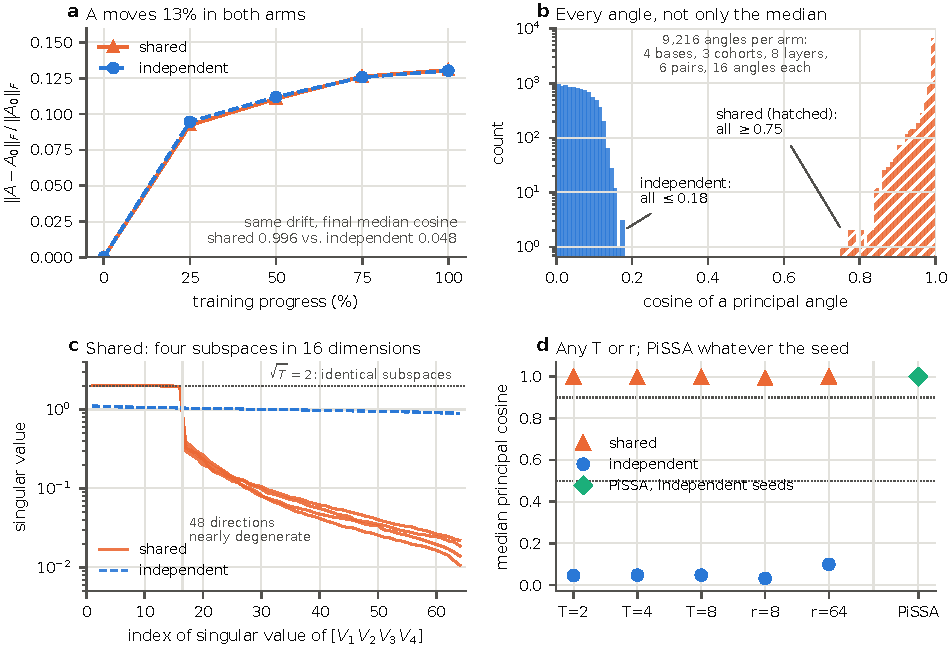
\includegraphics[width=\textwidth]{nc/figures/fig1_collapse.pdf}
\caption{What a shared initialisation does to a cohort. \textbf{(a)} Relative
displacement of $A$ from its initial value during training, on the Llama-3.1-8B
cohorts whose $A_0$ was saved: the two arms move by the same amount.
\textbf{(b)} Every principal cosine between every pair of task subspaces, at
$T = 4$, $r = 16$, pooled over four bases, three cohorts per arm and eight
layers (log count). \textbf{(c)} Singular values of the stacked orthonormal
bases $[V_1\,V_2\,V_3\,V_4]$, median over layers, one line per base: on the
shared arm $16$ values sit at $\sqrt{T} = 2$ and the other $48$ are small.
\textbf{(d)} Median principal cosine on Llama-3.1-8B across task count and
rank, and for a PiSSA cohort trained with four independent seeds. Dotted lines
in (d) mark the audit thresholds of \S\ref{subsec:audit}.}
\label{fig:collapse}
\end{figure}

\begin{table}[pos=tbp]
\centering
\small
\caption{The two regimes at $T = 4$, $r = 16$. The independent arm is the
first of three independent cohorts; the other two agree to three decimals.
Amplification is the norm of the exact interpolator over that of the mean task
update; $T = 4$ is its value for exactly orthogonal subspaces.}
\label{tab:regimes}
\begin{tabular}{lcccccc}
\toprule
 & \multicolumn{2}{c}{median cosine} & \multicolumn{2}{c}{$\kappa(\bar H)$}
 & \multicolumn{2}{c}{amplification} \\
base & shared & indep. & shared & indep. & shared & indep. \\
\midrule
Llama-3.1-8B & 0.995 & 0.047 & $1.76\times10^{4}$ & 1.5 & 48.3 & 4.0 \\
Mistral-7B   & 0.995 & 0.047 & $3.21\times10^{4}$ & 1.5 & 52.3 & 4.0 \\
Qwen2.5-7B   & 0.996 & 0.050 & $2.42\times10^{4}$ & 1.6 & 43.4 & 4.0 \\
Yi-1.5-9B    & 0.997 & 0.047 & $8.30\times10^{4}$ & 1.5 & 64.1 & 4.0 \\
\bottomrule
\end{tabular}
\end{table}

The separation is large and reproducible (Table~\ref{tab:regimes}). On every
base the shared cohort sits at a median principal cosine between $0.995$ and
$0.997$ and the independent cohorts between $0.047$ and $0.050$; the three
independent cohorts agree with each other to three decimals. It holds for every
principal angle, not only the median (Figure~\ref{fig:collapse}b): of the
$9{,}216$ principal cosines on each arm, every shared one is at least $0.75$
and every independent one at most $0.18$. The spectrum of the stacked subspace
bases shows where the dimensions go (Figure~\ref{fig:collapse}c). On the
shared arm, $16$ singular values sit near $\sqrt{T} = 2$ ($1.94$ to $1.96$),
the value for exactly identical subspaces, and the other $48$ fall from $0.3$
to $0.4$ down to $0.01$ to $0.02$, so four rank-$16$ subspaces occupy about
$16$ dimensions. On the independent arm all $64$ lie between $0.88$ and
$1.13$.

The subspaces are near-collinear, not collinear. Four rank-$16$ subspaces in
dimension $d = 4096$ remain linearly independent unless they coincide exactly,
so an exact interpolator exists in both regimes. The regimes differ in how
hard it is to reach. On the shared arm $\kappa(\bar H)$ is $1.8\times10^{4}$
to $8.3\times10^{4}$, against $1.5$ to $1.6$ on the independent arm, and the
exact interpolator is $43$ to $64$ times larger than the mean task update,
against $4.0$. That last value is $T$, the amplification for exactly orthogonal
subspaces, which the independent arm reproduces to within $1.1\%$. The
condition number depends on the curvature model behind $\bar H$, here the
projector model of \S\ref{sec:background}; the principal cosines do not, since
they are properties of the row spaces alone. That is why we lead with them.

\subsection{Task count, rank, training and initialisation scheme}\label{subsec:tr}

The argument above does not depend on $T$ or $r$, so the collapse should hold
at any size, and the conditioning should worsen as more subspaces crowd around
the same start. We tested both on Llama-3.1-8B, training adapters for four
further tasks (Dolly, XSum, CodeAlpaca and English-to-French translation) and
at ranks $8$ and $64$, in both arms. The regime is set by initialisation at
every size (Figure~\ref{fig:collapse}d): shared cohorts sit at median cosine
$0.990$ to $0.999$ and independent ones at $0.032$ to $0.099$. On the shared
arm the conditioning grows with the task count,
$\kappa(\bar H) = 3.9\times10^{3}$, $1.1\times10^{4}$ and $3.9\times10^{4}$ at
$T = 2, 4, 8$, and with the rank, $5.6\times10^{3}$, $1.1\times10^{4}$ and
$4.1\times10^{4}$ at $r = 8, 16, 64$, while on the independent arm the
amplification stays at the orthogonal value $T$ ($1.99$, $4.00$, $7.91$).

No change to training that we tried leaves the regime. We registered seven changes to
training on a shared-initialisation cohort of Llama-3.1-8B, each chosen to move
$A$ further or less far: the learning rate divided or multiplied by $3$, one or
four epochs instead of two, $A$'s learning rate multiplied by $4$, LoRA+ at
its recommended ratio of $16$ between the learning rates of $B$ and $A$, and
$A$'s initial value scaled by $0.25$. Every one stays collapsed, at median
cosine $0.956$ to $0.999$, and the independent counterparts of the two changes
expected to move $A$ furthest stay at $0.047$ and $0.048$. \S\ref{sec:theory} uses these
cohorts to test the theory out of sample, and reports one of them, a smaller
initial $A$, that stays collapsed but lowers the damage to a solver.

A shared seed is not the only route into the regime. PiSSA~\citep{meng2024pissa}
initialises $A$ from the principal singular vectors of the base weight, which
do not depend on the seed. Four PiSSA adapters trained with the independent
arm's four seeds form a collapsed cohort, at median cosine $0.999$, and their
trained row spaces remain at principal cosine $0.9996$ to the base weight's
top-$r$ right singular vectors: training does not move them far enough to
leave the starting subspace.

\subsection{Routes into the regime in practice}\label{subsec:routes}

\paragraph{Library defaults.} Whether two runs create the same $A$ is decided
by what the fine-tuning library does before it creates the adapter, which
\S\ref{subsec:libraries} reads from the source of two widely used stacks. We also
measured it. We fine-tuned Llama-3.2-1B-Instruct on GSM8K and on Alpaca with
Unsloth (2026.5.2) and with LLaMA-Factory (0.9.5), each at its default
settings, twice per task in separate processes. Within each library the
initial $A$ is identical across the two tasks and across the two runs (median
principal cosine $1.000$). After $50$ steps the two tasks' adapters remain at
$0.9996$ under Unsloth and $0.9994$ under LLaMA-Factory. A user who fine-tunes
several tasks with either library without changing its seed obtains a
collapsed cohort.

\paragraph{Continued training.} A common way to build several task adapters is
to start each from an adapter that already exists. We initialised four task
adapters from the $A$ and $B$ of one existing adapter (a Dolly instruction
adapter) and trained each with its own seed, so that no seed is shared. The
cohort is collapsed, at median cosine $0.997$ and
$\kappa(\bar H) = 2.9\times10^{4}$, and adapter-only RegMean at
$\lambda = 10^{-6}$ leaves a worst-task excess of $1.49$ nats, against $0.071$
on the independent cohort of the main grid. Derived adapters reach the regime
without any seed in common.

\paragraph{Other parameterisations and a vision model.} Weight-decomposed LoRA
(DoRA) keeps a LoRA-style $A$, and a shared seed collapses it in the same way:
median cosine $0.995$ for a shared cohort and $0.047$ for an independent one
on Llama-3.1-8B. We measured geometry only, since merging DoRA needs a
treatment of its magnitude vector that this pipeline does not have. Rank-stabilised
LoRA draws $A$ from the same distribution and changes only the scaling, so its
collapse at creation is identical by construction. The regime is not specific
to language models either: rank-$16$ adapters on CLIP ViT-B/32, trained on
eight image classification tasks, sit at median cosine $0.96$ in shared
cohorts and $0.11$ in independent ones (\S\ref{subsec:beyond}).


\section{A first-order theory of the collapse}\label{sec:theory}
Section~\ref{sec:collapse} measured a four-order-of-magnitude rise in
$\kappa(\bar H)$ and a ten-fold rise in the interpolator's norm. This section
derives both from one assumption, that each adapter's $A$ factor is a small
displacement of a common start. It then tests the derivation against the
adapters, and tests a scalar law derived from it on training regimes it was
not calibrated on.

\paragraph{Set-up.} In a shared cohort, $A_t = A_0 + E_t$. Let
$W_0 \in \R^{d\times r}$ be an orthonormal basis of the row space of $A_0$ and
$P_\perp = I - W_0 W_0^\top$. Whenever $W_0^\top A_t^\top$ is invertible, the
row space $V_t$ of $A_t$ is exactly the graph of a \emph{tilt}
\begin{equation}\label{eq:tilt}
  X_t \;=\; P_\perp A_t^\top \bigl(W_0^\top A_t^\top\bigr)^{-1} \in \R^{d\times r},
  \qquad V_t = \operatorname{col}(W_0 + X_t),
\end{equation}
and the principal angles between $V_t$ and the starting subspace satisfy
$\tan\theta_i = \sigma_i(X_t)$. The tilt is of the order of the relative
displacement:
\[
  \|X_t\| \;\lesssim\; \|E_t\| / \sigma_{\min}(A_0).
\]
Write
$D_t = \Delta W_t$ for the task updates and $M_t = D_t(W_0 + X_t)$ for their
action on the tilted bases.

\begin{proposition}[First-order conditioning of a shared cohort]
\label{prop:drift}
Let $Y = [X_1 - \bar X, \dots, X_T - \bar X] \in \R^{d\times Tr}$ collect the
centred tilts and $\Sigma_X = \tfrac1T Y Y^\top$. To leading order in the tilt,
\begin{enumerate}[leftmargin=*,itemsep=1pt,topsep=2pt]
\item $\bar H$ has $r$ eigenvalues $1 - O(\|X\|^2)$ and $(T-1)r$ eigenvalues
  equal to the nonzero eigenvalues of $\Sigma_X$, so
  $\kappa(\bar H) \approx 1/\lambda_{\min}^{+}(\Sigma_X)$;
\item the exact interpolator is $\tauH \approx a\,W_0^\top + b$ with
  $b = [M_1 - \bar M, \dots, M_T - \bar M]\, Y^{+}$ and $a = \bar M - b\bar X$;
\item under a uniform rescaling of the displacements $E_t \mapsto sE_t$,
  $\kappa(\bar H) \propto s^{-2}$ while the amplification
  $\|\tauH\|/\|\bar D\| \propto s^{-1}$.
\end{enumerate}
\end{proposition}

The derivation, in Appendix~\ref{app:theory}, expands each projector to second
order in $X_t$ and takes the Schur complement of $\bar H$ on the orthogonal
complement of the starting subspace. The interpolation conditions
$\tauH(W_0 + X_t) = M_t$ then separate into a component along $W_0$ and one
along the centred tilts. In words: the subspaces share $r$ directions almost
exactly, those directions are well conditioned, and everything else a merge
must resolve lives in the small differences between the tilts.
Figure~\ref{fig:theory}a shows this on a real layer: the prediction follows
the exact spectrum of $\bar H$ across all $48$ small eigenvalues, not only at
the smallest one that sets $\kappa$.

\paragraph{A consequence.} The amplification is of first order in the inverse
displacement and $\kappa$ of second order. And $\kappa(\bar H)$ is set by the
\emph{smallest} singular value of the spread of the displacements, not by
their size. A displacement of $13\%$ in every direction would give
$\kappa \approx 60$. The measured $10^{4}$ to $10^{5}$ therefore means that
training displaces the adapters very unevenly, leaving some directions of the
spread almost unexcited. On synthetic cohorts the same relative displacement
gives $\kappa \approx 5\times10^{2}$ with isotropic displacements and $10^{5}$
to $10^{6}$ with low-rank ones (Appendix~\ref{app:theory}).

\paragraph{Tests.} We registered five predictions before computing any of the
quantities involved, and all five hold (Figure~\ref{fig:theory}).
\begin{itemize}[leftmargin=*,itemsep=1pt,topsep=2pt]
\item \emph{The conditioning, during training.} On a Llama-3.1-8B cohort whose
  $A_0$ was saved before the first optimiser step, the first-order prediction
  of $\kappa(\bar H)$ equals the exact value at $25$, $50$, $75$ and $100\%$
  of training.
\item \emph{The amplification, during training.} The same holds for the
  amplification on the same cohort and checkpoints.
\item \emph{The formula, without $A_0$.} A reference-free version, which takes
  the consensus subspace of the cohort as $W_0$ and needs no saved start, does
  the same on all twelve shared cohorts of the four bases, and on the five
  task-count and rank configurations of \S\ref{subsec:tr}.
\item \emph{The orders.} Rescaling the measured displacements by five factors
  $s$ from $0.05$ to $1$ gives exact log-log slopes of $-2.00$ for
  $\kappa$ and $-1.01$ for the amplification, inside the registered bands
  $[-2.2, -1.8]$ and $[-1.2, -0.8]$. The rival $s^{-2}$ form for the
  amplification is excluded.
\item \emph{Across training.} Both quantities fall monotonically as the
  adapters drift, $\kappa$ from $2.7\times10^{4}$ to $1.1\times10^{4}$ and the
  amplification from $61$ to $44$.
\end{itemize}
Across the $21$ configurations, the predicted $\kappa(\bar H)$ lies between
$0.9990$ and $1.0005$ times the exact value, within $0.10\%$. The predicted
amplification matches to six digits, but that match is close to algebraic and
we do not count it as evidence: the interpolation conditions behind item~2 of
the proposition are exact, and the one approximation, dropping a coupling
through $\bar X$, vanishes for the consensus $W_0$ of the reference-free test.
The evidence for the expansion is the agreement of $\kappa$, which rests on the
second-order expansion of the projectors, and the two slopes.

\paragraph{Out of sample.} These tests compute each prediction from the same
adapters' tilts. A stronger test is whether the scaling of item~3 carries to
cohorts trained differently. Item~3 implies a scalar law,
$\kappa(\bar H) \approx C_\kappa / t^2$ and amplification $\approx C_a / t$,
where $t$ is the median over tasks and layers of the spectral norm of the tilt
$X_t$ under the consensus $W_0$. We fixed $C_\kappa$ and $C_a$ on the four
existing shared Llama-3.1-8B cohorts and committed them before training the
seven cohorts of \S\ref{subsec:tr} (learning rate, epochs, $A$'s learning
rate, LoRA+ and the scale of $A_0$), which with the baseline cohort trained
alongside them give eight test cohorts. The registered thresholds were a
factor of $2$ for $\kappa$ on at least six and a factor of $1.25$ for the
amplification on at least seven. The law predicts $\kappa$ within a factor of
$2$ on all eight, over a range from $1.2\times10^{3}$ to $5.5\times10^{4}$,
and the amplification within $1.25$ on seven. Across the eight cohorts $t$ and
$\kappa$ have Spearman correlation $-0.976$. Reaching the independent arm's
median $\kappa$ of $1.55$ would take a tilt of $t^\star = 22$, $27$ times the
largest tilt any regime produced ($0.83$). The shared cohorts trained at three
times the learning rate and at four times $A$'s learning rate leave
adapter-only RegMean at $\lambda = 10^{-6}$ with an excess of $0.34$ and
$0.38$ nats, against $0.057$ and $0.073$ for their independent counterparts.
All five predictions of this second registration hold, and it permits saying
that the scalar law predicts $\kappa$ on these regimes. That claim is limited
to one base model and to changes of training that keep a shared start.

One regime departs from the picture in a way we did not predict. Scaling
$A_0$ by $0.25$ before training gives the largest relative tilt ($0.83$),
$\kappa(\bar H) = 1.2\times10^{3}$, and an amplification of $7.5$, about half
the $13.7$ the law predicts; it is the one amplification miss. On this cohort
adapter-only RegMean at $\lambda = 10^{-6}$ leaves an excess of only $0.022$
nats, below the independent cohort's $0.071$. Three times the learning rate
reaches the same $\kappa$ ($1.2\times10^{3}$) with an amplification of
$15.9$, and there the excess is $0.34$. The two cohorts have equal $\kappa$
and differ in amplification, and the solver's damage differs with it. We note
this as an observation from two cohorts; a smaller initial $A$ as a mitigation
would need its own test.

\begin{figure}[pos=tbp]
\centering
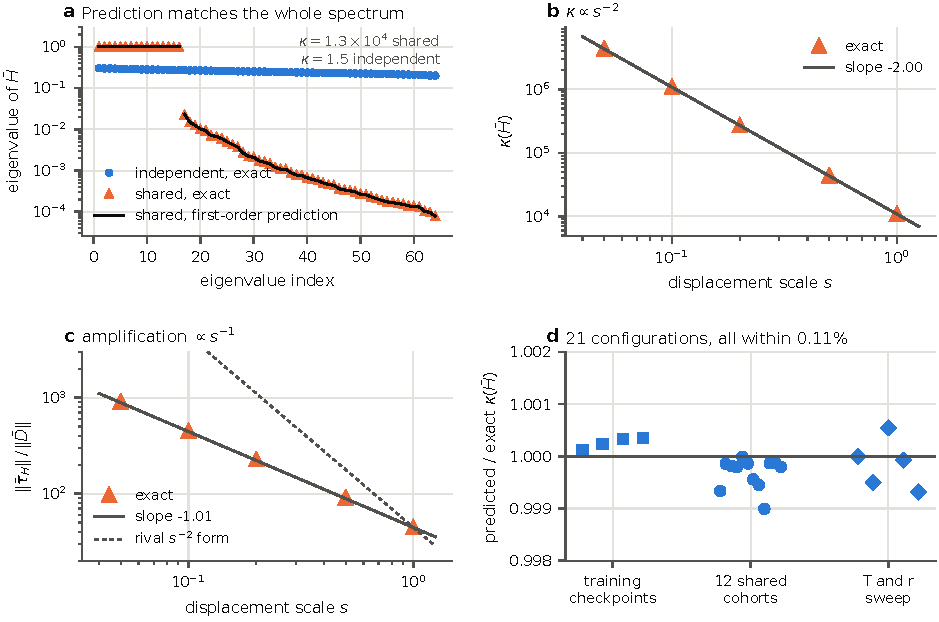
\includegraphics[width=\textwidth]{nc/figures/fig2_theory.pdf}
\caption{The first-order theory against exact values. \textbf{(a)} All $64$
eigenvalues of $\bar H$ for one layer of a Llama-3.1-8B cohort (the layer with
the median $\kappa$ of the eight sampled): on the shared cohort, $r = 16$
eigenvalues sit at $1$ and the other $48$ follow the eigenvalues of
$\Sigma_X$ that Proposition~\ref{prop:drift} predicts (line); on the
independent cohort all $64$ sit near $1/T$. \textbf{(b, c)} The displacements
of a shared cohort rescaled by $s$; lines have the fitted slopes, and the dashed
line in (c) is the rival $s^{-2}$ form, which the data exclude.
\textbf{(d)} Predicted over exact $\kappa(\bar H)$ at four training
checkpoints, on twelve shared cohorts of four bases, and at five task counts
and ranks. All $21$ ratios lie in $[0.9990, 1.0005]$.}
\label{fig:theory}
\end{figure}

\paragraph{Scope.} The proposition is a leading-order expansion
checked numerically, not a bound with explicit constants. It describes the
shared regime only; in the independent regime the tilts are not small and the
amplification equals $T$ by a separate identity. It explains the
conditioning a solver would face, and its scalar form predicts that
conditioning across the training regimes we tested; whether a given solver
faces it is the question of \S\ref{sec:merging}.


\section{Where the collapse occurs}\label{sec:prevalence}
\subsection{A pre-merge audit}\label{subsec:audit}

Everything in \S\ref{sec:collapse} is computed from the adapter weights, so the
regime of a cohort can be read before any merge is attempted.
Algorithm~\ref{alg:audit} does it. It reads only the $A$ factors: no $B$
factors, no base weights, no forward passes and no data. Its cost is
$O(T^2 r^2 d)$ per layer, about one CPU minute for four rank-$16$ adapters over
eight layers. The thresholds were fixed before any public cohort was measured
and are used unchanged throughout.

\begin{algorithm}[t]
\caption{Pre-merge audit of a LoRA cohort.}
\label{alg:audit}
\begin{algorithmic}[1]
\Require adapters $\{A_t\}_{t=1}^{T}$ on a common base; a sample of layers
  $\mathcal{L}$; thresholds $c_{\mathrm{hi}} = 0.9$, $c_{\mathrm{lo}} = 0.5$
\State $C \gets \emptyset$
\For{each layer $\ell \in \mathcal{L}$}
  \State $V_t \gets \mathrm{orth}\bigl(A_t^{(\ell)\top}\bigr)$ for each $t$
    \Comment{orthonormal basis of the row space}
  \For{each pair $i < j$}
    \State $C \gets C \cup \operatorname{svals}\bigl(V_i^{\top} V_j\bigr)$
      \Comment{cosines of the principal angles}
  \EndFor
\EndFor
\State $\bar c \gets \operatorname{median}(C)$
\State \Return \textsc{collapsed} if $\bar c > c_{\mathrm{hi}}$,
  \textsc{separated} if $\bar c < c_{\mathrm{lo}}$, else \textsc{indeterminate}
\end{algorithmic}
\end{algorithm}

A cohort cannot be repaired by editing its $A$ factors while keeping each
adapter's behaviour. Replacing $A_t$ by $QA_t$ for an invertible $Q$ preserves
the adapter only if $B_t$ becomes $B_tQ^{-1}$, and then the row space, the
principal cosines and $\bar H$ are all unchanged. The geometry is a property of
what the adapters compute, so only retraining or the choice of merge can
change what it does to a merge.

\subsection{Which fine-tuning stacks produce the collapse}\label{subsec:libraries}

Whether two adapters receive the same initial $A$ is decided by library code,
so we read it. In PEFT (version 0.19.1, which wrote all our adapters), the
default initialisation draws $A$ with \texttt{kaiming\_uniform\_} from the
global PyTorch generator; PEFT takes no per-adapter seed and does not reseed.
Two runs therefore receive identical $A$ exactly when the generator is in the
same state as each layer is built: the same seed set beforehand, the same
target modules in the same order at the same rank, and the same device and
data type. Nothing about the task or the data enters.

The question is then what runs before the adapter is created. We read two
widely used fine-tuning stacks at pinned versions. Unsloth~\citep{unsloth2026}
(2026.5.2) gives \texttt{get\_peft\_model} a default \texttt{random\_state} of
$3407$ and sets the seed with it before creating the LoRA layers.
LLaMA-Factory~\citep{zheng2024llamafactory} sets the training seed, $42$ by
default, before the model is loaded. At their defaults both stacks therefore
give every run on one base, target set and rank the same initial $A$: a user
who fine-tunes several tasks without changing the seed obtains a collapsed
cohort. TRL's \texttt{SFTTrainer} builds the PEFT model before it seeds, so its
behaviour depends on the calling script, and we found no seeding before
adapter creation in axolotl. Without any seed the regime does not arise by
accident, since fresh processes start the generator differently. This is a
reading of source code, not a measurement.

\subsection{Prevalence in public adapters}\label{subsec:public}

Our own cohorts say nothing about anyone else's, so we ran the audit on public
cohorts under a protocol registered before any adapter was downloaded. We
walked the HuggingFace model index filtered to PEFT and sorted by downloads,
which weights the sample towards adapters that are used, and grouped adapters
into cohorts by publisher and base model. A cohort entered if it had at least
two readable LoRA adapters of rank at least $4$ on one base, sharing a target
module. Every criterion was checked from metadata before any weight was
fetched, and no cohort was skipped after inspection. We walked $1000$ models to
reach the registered $50$ cohorts; five could not be scored, leaving $45$.

\begin{figure}[pos=tbp]
\centering
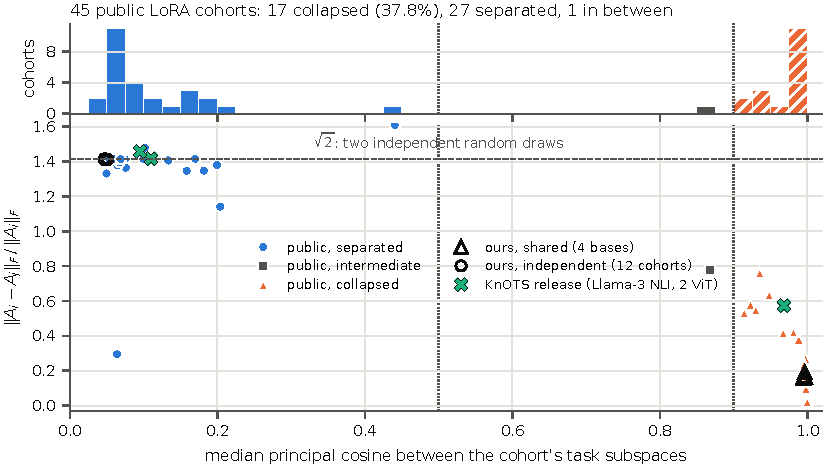
\includegraphics[width=\textwidth]{nc/figures/fig3_prevalence.pdf}
\caption{The $45$ public LoRA cohorts, sampled by a frame registered before
any download. Horizontal axis: median principal cosine between the cohort's
task subspaces, with the audit thresholds dotted and its histogram on top.
Vertical axis: relative distance between the cohorts' $A$ factors, which is
$\sqrt 2$ for two independent random draws. Two cohorts whose members differ in
rank have no distance and appear only in the histogram. Open markers are our
own cohorts; crosses are the three cohorts released with KnOTS, the one merging
paper among $22$ checked that releases LoRA cohorts.}
\label{fig:prevalence}
\end{figure}

Seventeen of the $45$ cohorts, $37.8\%$, are collapsed; the registered
prediction was $20\%$. The distribution is bimodal rather than a continuum cut
by a threshold (Figure~\ref{fig:prevalence}): $27$ cohorts are separated, with
median cosine $0.076$, and only one falls between the thresholds, at $0.868$.
An unplanned check supports the measurement. If two adapters draw $A$
independently and $A$ moves little, then
$\|A_i - A_j\|_F \approx \sqrt2\,\|A_i\|_F$. The separated cohorts give a
median ratio of $1.414$, as independent draws should, while the collapsed
cohorts range from $0.017$, adapters whose $A$ factors agree to within
$1.7\%$, to $0.760$ (Figure~\ref{fig:prevalence}, vertical axis). One separated
cohort sits at only $0.29$, the single point this check does not explain. Our
own cohorts and the three released with KnOTS (below) fall inside the two
public clusters.

The cohorts that merging papers evaluate on are harder to sample. We checked the
$22$ merging papers we cite in order, intending to audit the first two that
release LoRA cohorts; only one does. KnOTS~\citep{stoica2025knots} releases a
Llama-3-8B cohort of six natural-language-inference adapters and two vision
cohorts. Its language cohort is collapsed, at median cosine $0.968$, and its
vision cohorts are separated, at $0.110$ and $0.095$. A released cohort that a
later merging paper uses as its benchmark~\citep{panariello2025core} is
therefore in the collapsed regime. This is a single paper, so we draw no
conclusion about merging benchmarks in general.


\section{Which merges the collapse affects}\label{sec:merging}
A collapsed cohort makes $\bar H$ badly conditioned. Whether that matters
depends on whether a merge ever solves against a matrix that inherits it. This
section tests that on twelve methods, ten of them published methods we did not
build. It compares every method with itself across the two regimes and reports
NLL for every method and downstream accuracy for all but one. It then repeats the central comparisons on a
vision model and on the two tasks not yet scored, and asks whether the ridge
can be set without data.

\subsection{The prediction}\label{subsec:prediction}

Before running the methods we did not build, we registered which of them the
mechanism says are exposed. An averaging or sparsifying merge forms a
combination of the task updates and never solves against $\bar H$, so it
should not care. A solver is exposed if the matrix it inverts is built from
the adapters themselves, because that matrix inherits the collapse. A solver
whose matrix is built from data, such as input activations or a Fisher
estimate, inverts something the initialisation does not control, and a
diagonal matrix cannot see overlap between subspaces at all. Whitening the
stacked singular vectors of the task updates (TSV-M) was predicted to be
exposed, since it too inverts a matrix built from the updates.

WUDI-Merging~\citep{cheng2025wudi} is the one published data-free method we
found whose least-squares matrix is built from the task updates, so the rule
places it in the exposed class. Its authors do not solve that system, however.
They minimise its objective with $300$ steps of Adam started from the sum of
the task updates, and an early-stopped gradient method acts as an implicit
ridge. We therefore registered a split prediction: the closed form would be
exposed and the published procedure protected by its optimiser. We also wrote
in advance that if the published procedure failed, that would become the lead
result of this paper.

\subsection{A published data-free merge fails}\label{subsec:wudi}

For each linear layer, WUDI-Merging minimises
\begin{equation}\label{eq:wudi}
  \mathcal{L}(\tau) = \sum_{t=1}^{T}
  \frac{\|(\tau - D_t)\,D_t^\top\|_F^2}{\|D_t\|_F^2},
\end{equation}
where $D_t = s\,B_tA_t$ is the update of task $t$ and $s$ the LoRA scaling.
The matrix of this least-squares problem is
$\sum_t D_t^\top D_t / \|D_t\|_F^2$. For a LoRA update its range is the row
space of the $A_t$, which is exactly the subspace the collapse shrinks. We ran
three versions on all six cohorts of the four bases. The first is the authors'
procedure as their code runs it: Adam with learning rate $10^{-5}$, no weight
decay, $300$ steps, started at $\sum_t D_t$. The second is the closed form of
their Eq.~(20) with $\omega = 10^{-6}$, solved in float64. The third is the
published procedure run for $3000$ steps, as a dose arm. Each merged update was
truncated to rank $r$ like every other merge. We evaluate the loss from the
factors rather than densely; it is the same function, and we checked its value,
gradient and a $50$-step Adam trajectory against the dense form.

\begin{table}[pos=tbp]
\centering
\small
\caption{WUDI-Merging on shared and independent cohorts, three per arm.
\emph{NLL ratio}: mean worst-task excess on the shared arm over that on the
independent arm; every ratio clears the registered gate. Accuracy is the mean
over three cohorts, shared / independent. $^\dagger$Within the gate; every
other accuracy difference clears it.}
\label{tab:wudi}
\setlength{\tabcolsep}{4pt}
\begin{tabular}{lccccccc}
\toprule
 & \multicolumn{3}{c}{NLL ratio, shared / indep.}
 & \multicolumn{2}{c}{as published}
 & \multicolumn{2}{c}{closed form} \\
\cmidrule(lr){2-4}\cmidrule(lr){5-6}\cmidrule(lr){7-8}
base & published & closed form & 3000 steps & GSM8K & HumanEval & GSM8K & HumanEval \\
\midrule
Llama-3.1-8B & 14.9 & 30.7 & 22.7 & 0.034 / 0.695 & 0.000 / 0.526 & 0.056 / 0.701 & 0.096 / 0.537 \\
Mistral-7B   & 47.6 & 65.1 & 60.5 & 0.001 / 0.251 & 0.000 / 0.057 & 0.003 / 0.267 & 0.000 / 0.049$^\dagger$ \\
Qwen2.5-7B   &  6.3 &  7.8 & 10.1 & 0.479 / 0.619 & 0.567 / 0.665$^\dagger$ & 0.180 / 0.625 & 0.459 / 0.685 \\
Yi-1.5-9B    &  4.7 &  5.3 &  4.7 & 0.205 / 0.717 & 0.014 / 0.124 & 0.094 / 0.717 & 0.000 / 0.130 \\
\bottomrule
\end{tabular}
\end{table}

The published procedure fails (Table~\ref{tab:wudi}). Its worst-task excess is
$14.9$, $47.6$, $6.3$ and $4.7$ times larger on the shared arm than on the
independent arm on Llama, Mistral, Qwen and Yi, past the gate on every base,
so the prediction that the optimiser protects it fails on all four. Accuracy
follows. On GSM8K the shared cohorts score $0.034$, $0.001$, $0.479$ and
$0.205$ against $0.695$, $0.251$, $0.619$ and $0.717$ on the independent ones.
On HumanEval the shared arm is worse past the gate on three of four bases, and
on Llama and Mistral it scores zero in every shared cohort. The closed form is
exposed as predicted: $5.3$ to $65$ times worse in NLL, and worse on GSM8K on
every base. On independent cohorts all three versions leave a worst-task
excess of only $0.03$ to $0.16$ nats.
A practitioner who runs WUDI as published on a collapsed cohort gets a broken
model and no warning.

The account we registered of how this happens did not hold. We predicted that
the closed form would put at least half of its energy in the bottom quarter of
$\bar H$'s spectrum, as the two solvers of \S\ref{subsec:results} do. It puts
$0.03$ to $0.17$ there on the shared arm, less than on the independent arm. We
also predicted that the 3000-step arm would fall between the other two, and it
does not on two of the four bases: it lies above the closed form on Qwen and
below the published version on Yi. Two diagnostics that we recorded but did not
register as mediators separate the arms for the published procedure. The
first is how far Adam moves. The starting sum has exactly $T = 4$ times the
norm of the mean update. On independent cohorts Adam leaves it there
(amplification $4.0$), and on shared cohorts it drives it to $8.6$ to $12.5$.
The second is where the movement goes. On the shared arm, $24$ to $27\%$ of
the merged update's squared norm lies outside the row space of the $A_t$,
against $0.8$ to $1.6\%$ on the independent arm. The loss in
Eq.~\eqref{eq:wudi} cannot see that component, because it depends on $\tau$
only through $\tau D_t^\top$. A reading consistent with both diagnostics is
as follows. On near-orthogonal subspaces the sum already minimises the loss,
since $D_sD_t^\top \approx 0$ for $s \neq t$, so there is little gradient. On a
collapsed cohort the sum counts the shared directions about four times, the
loss is far from its minimum, and Adam moves far. Because Adam rescales each
coordinate separately, its steps leave the row space, and the loss never
corrects what lands outside it. We offer this as a description, not as a
tested mechanism.

\subsection{Where each merge puts its energy}\label{subsec:energy}

\begin{figure}[pos=tbp]
\centering
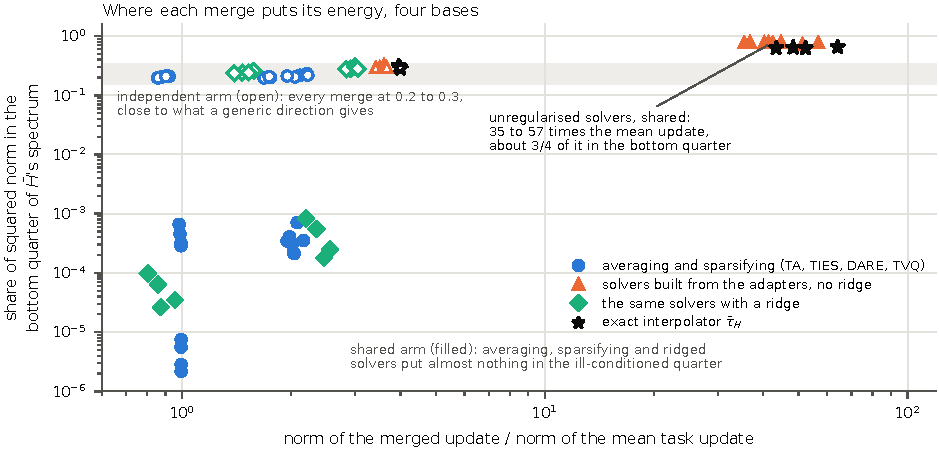
\includegraphics[width=\textwidth]{nc/figures/fig4_mechanism.pdf}
\caption{Where each merged solution puts its energy, on the four bases. Each
point is one method on one base; filled markers are the shared cohort, open
markers the independent one. Horizontal: norm of the merged update relative to
the mean task update. Vertical: share of its squared norm in the bottom quarter
of $\bar H$'s spectrum, the ill-conditioned directions. ``The same solvers with
a ridge'' are adapter-only RegMean at $\lambda = 0.13$ and our encoder at its
selected $\lambda$.}
\label{fig:mechanism}
\end{figure}

For the other methods the mechanism can be checked without any forward pass,
because every merge is arithmetic on the adapter factors
(Figure~\ref{fig:mechanism}). On the shared arm, every averaging and
sparsifying merge has a norm $0.98$ to $2.16$ times that of the mean task
update. The share of its energy in the bottom quartile of $\bar H$'s spectrum
rounds to $0.000$. The two unregularised solvers built from the adapter
factors have norms $35$ to $57$ times the mean update and put $73$ to $80\%$
of their energy there. Among these methods they are the only ones that enter
the ill-conditioned directions, and a ridge brings them back down beside the
heuristics. On the independent arm every method puts $0.19$ to $0.32$ of its
energy in the bottom quarter, close to what a direction unrelated to the
spectrum gives. WUDI is the exception to this picture
(\S\ref{subsec:wudi}): it is amplified on the shared arm without
concentrating in those directions.

\subsection{The other methods}\label{subsec:results}

\begin{table}[pos=tbp]
\centering
\small
\caption{Which merges the collapse reaches. Each method is compared with itself
on shared and independent cohorts, three per arm on four bases. NLL is the
ratio of worst-task excess, shared over independent, over the four bases.
Accuracy is GSM8K exact match and HumanEval pass@1; for MaTS it uses one cohort
per arm. KnOTS is its TIES variant, and diagonal Fisher uses the squared update
as a data-free proxy for the Fisher. The prediction was registered before any
of the methods we did not build was run.}
\label{tab:exposure}
\setlength{\tabcolsep}{3.5pt}
\begin{tabularx}{\textwidth}{>{\raggedright\arraybackslash}p{2.5cm}
                >{\raggedright\arraybackslash}p{1.7cm}
                >{\raggedright\arraybackslash}p{1.5cm}
                >{\raggedright\arraybackslash}X
                >{\raggedright\arraybackslash}X}
\toprule
method & matrix built from & predicted & NLL, shared / indep. & accuracy \\
\midrule
task arithmetic, TIES, DARE, TVQ, KnOTS & no matrix & immune
  & no effect in 15 of 20 cells; largest $0.015$ nats
  & equivalent within $3$ points (GSM8K) and $5$ (HumanEval) \\
\addlinespace
RegMean, activation Grams & data & immune & $0.99$ to $1.14$
  & equal in 8 of 8 cells \\
MaTS & data (Fisher) & immune & $0.93$ to $0.99$
  & equal in 7 of 8; 1 favours shared \\
diagonal Fisher & task updates, diagonal & immune & $0.96$ to $1.08$ & not run \\
\addlinespace
TSV-M (whitening) & task updates & exposed & $0.81$ to $1.19$, mixed sign
  & no cell past the gate \\
\addlinespace
WUDI, as published & task updates & protected by its optimiser & $4.7$ to $47.6$
  & GSM8K $0.00$ to $0.48$ vs.\ $0.25$ to $0.72$ \\
WUDI, closed form & task updates & exposed & $5.3$ to $65.1$
  & GSM8K $0.00$ to $0.18$ vs.\ $0.27$ to $0.72$ \\
\addlinespace
RegMean, adapter-only & adapter factors & exposed & $1.8$ to $65.6$
  & GSM8K $0.00$ to $0.17$ vs.\ $0.29$ to $0.72$ \\
our encoder & adapter factors & exposed & $2.8$ to $76$
  & Mistral $0.000$ on both \\
\bottomrule
\end{tabularx}
\end{table}

\begin{figure}[pos=tbp]
\centering
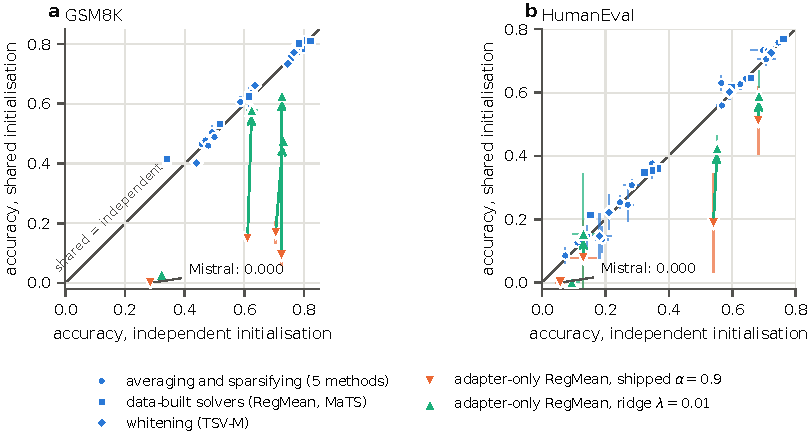
\includegraphics[width=\textwidth]{nc/figures/fig5_accuracy.pdf}
\caption{Downstream accuracy on shared against independent cohorts. Each point
is one method on one base model, the mean over three cohorts per arm, with bars
of one standard deviation across cohorts. Points on the diagonal are unaffected
by the initialisation. Every published method shown lies on or near it;
adapter-only RegMean at its shipped setting ($\alpha = 0.9$) lies far below it.
Arrows go from that setting to the same solver with a ridge of
$\lambda = 0.01$ on the same base, which recovers most of the loss on three
bases and not on Mistral. WUDI is in Table~\ref{tab:wudi}.}
\label{fig:exposure}
\end{figure}

Table~\ref{tab:exposure} and Figure~\ref{fig:exposure} give the outcome for
every method.

\paragraph{Averaging and sparsifying merges are unaffected.} In NLL, $15$ of
$20$ base-by-method cells show no difference that clears the registered gate.
The gate is the larger of $0.005$ nats and twice the standard error, and sits
near $0.01$ nats. The five that do are small and favour the independent arm.
Three of them are the subspace-aligning KnOTS, the heuristic that operates most
directly on subspace geometry. Because a null at hundredths of a nat is weak
evidence, we registered the accuracy comparison as an equivalence test (two
one-sided tests, three cohorts per arm, $240$ cells). All five heuristics are
equivalent across regimes within the registered margins of $3$ points on GSM8K
and $5$ on HumanEval, and each would pass at $0.9$ to $2.0$ points and $2.1$ to
$3.0$ points respectively. The equivalence is a statement about means over the
four bases. One of $40$ cells taken alone exceeds its margin: TIES on Llama at
HumanEval, where the shared arm is $6.5$ points higher.

We also registered that a slight lean towards the shared arm, seen at one
cohort per arm, would vanish at three. It persisted: $29$ of the $38$ non-zero
differences favour the shared arm (sign test, $p = 0.0017$). That test treats
the $40$ cells as independent, although the ten cells of a base share its six
cohorts and its evaluation sets. A permutation test that we ran afterwards,
which relabels whole cohorts within each base, gives $p = 0.007$ for a mean
lean of $0.7$ points, with all four bases leaning the same way. We tested one
explanation in advance. Truncation to rank $r$ discards more of an independent
cohort's merged update: $12$ to $25\%$ of task arithmetic's squared norm,
against $1.3$ to $1.6\%$ on the shared arm, and more on the independent arm for
every heuristic on every base. Merging without truncation should then have
halved the lean. It did not halve on any of the three method-benchmark pairs
where the lean was largest (task arithmetic and DARE at HumanEval, TIES at
GSM8K), so truncation is excluded as its cause. No heuristic enters the
ill-conditioned directions, so the lean is not the solver mechanism either,
and we have no tested explanation for it. In practice, a heuristic merge loses
nothing to a shared initialisation.

\paragraph{Solvers built from data, and a diagonal one, are unaffected.}
RegMean with real activation Grams at its published setting, MaTS with its
blockwise Fisher solved by conjugate gradient, and diagonal Fisher merging were
run on all three cohorts of both arms on all four bases. Our diagonal Fisher
weights each coordinate by its squared update, a data-free proxy, so its matrix
comes from the task updates; being diagonal, it cannot see overlap between
subspaces. The three immunity predictions hold. RegMean shows no effect on any base in either unit and is the most
accurate merge in our experiments on every base; its accuracy on the two arms
agrees within $1.3$ points in all eight base-by-benchmark cells. MaTS shows no
NLL effect, and in accuracy one cell (Mistral, GSM8K) favours the shared arm.
Diagonal Fisher shows one small effect, $1.08$ times on Llama. A practitioner
who has the data RegMean was designed for is unaffected by the collapse.

\paragraph{Whitening is not affected, against our prediction.} TSV-M was
predicted to be exposed. It shows an NLL effect on Mistral only ($1.19$ times),
one in the opposite direction on Yi, and none on Llama and Qwen, and no
accuracy cell clears the gate. The prediction failed. Whitening orthogonalises
the stacked singular vectors rather than solving a least-squares problem in
them, and the rule in \S\ref{subsec:rule} is stated for least-squares merges
alone.

\paragraph{Solvers built from the adapter factors fail.} The data-free form of
RegMean replaces each activation Gram by $A_t^\top A_t$. It is a variant we
constructed, not the published method, and it is the natural choice when only
the adapter files are available. With a minimal ridge ($\lambda = 10^{-6}$) its
worst-task excess (Figure~\ref{fig:ridge}, top row) is $4.1$, $65.6$, $5.8$ and
$1.8$ times larger on the shared arm on Llama, Mistral, Qwen and Yi, and the
gain from tuning the ridge is larger on the shared arm on all four; both match
the registered predictions. In accuracy, with RegMean's own shipped regulariser
($\alpha = 0.9$) and no added ridge, the shared arm scores $0.168$, $0.000$,
$0.148$ and $0.093$ on GSM8K against $0.705$, $0.285$, $0.611$ and $0.724$ on
the independent arm. On Mistral it scores zero on both benchmarks in all three
shared cohorts. A ridge of $\lambda = 0.01$ beats the shipped setting on the
shared arm past the gate on three of four bases on GSM8K, by $31$, $43$ and
$54$ points on Llama, Qwen and Yi, and on two on HumanEval. It does not rescue
Mistral ($0.029$ and $0.002$), whose NLL sweep selects $\lambda = 0.05$, so
$0.01$ is a starting point for a sweep rather than a recommended value.

The second solver of this kind is the closed-form encoder of our earlier
preprint~\citep{pathak2026rd}, which we call \emph{our encoder}. It computes
the exact interpolator $\tauH = \bar D\,\bar H^{+}$ of \S\ref{sec:background}
directly, with an optional ridge on the range of $\bar H$, so it inverts the
collapsed operator itself. Unregularised it is $2.8$ to $76$ times worse on
the shared arm (three cohorts per arm, every base past the gate), and on
Mistral its merged model scores $0.000$ on both benchmarks, recovering to
$0.46$ on GSM8K and $0.24$ on HumanEval with a tuned ridge. The effect
survives with rank truncation disabled, where the ratio grows to $25$ to
$117$: truncating to rank $r$ discards most of the ill-conditioned subspace and
so hides part of the damage. On both solvers, the amount of ridge that is
needed does not track the conditioning, while the amount it buys does; the
selected $\lambda$ is identical across the two arms on three of four bases for
the encoder and on two for adapter-only RegMean.

\paragraph{Numerical precision and truncation.} Both solvers run in float32,
and at $\lambda = 10^{-6}$ and $\lambda = 0$ their systems are badly
conditioned, so the failure could in principle be rounding error. We
registered a check before running it: for each base, arm and solver, recompute
the merge in float64 from the same adapter factors and compare the two after
exact truncation to rank $r$. Precision would be excluded if the median
difference over modules stayed below $1\%$ and the ratio of shared to
independent amplification changed by less than a factor of $2$. The ratios
agree within $0.1\%$ in every case, and $15$ of the $16$ medians are below
$1\%$, at most $0.9\%$. The encoder on the shared Yi cohort is at $1.09\%$ and
fails, so, as registered, we rebuilt that merge in float64 and evaluated it
again. Its worst-task excess is $0.245$ nats against $0.249$ in float32, and
$0.121$ on the independent cohort: rounding does not cause the failure. Runs
we added afterwards show that the float32 merge is unstable instead. The
encoder's per-task bases come from a randomised SVD, and the unregularised
solve amplifies its rounding, so float32 merges that differ only in the random
seed reach worst-task excesses of $0.22$ to $0.28$ nats on this cohort, and
$0.26$ to $0.84$ when the truncation to rank $r$ is exact. All of them lie
above the independent cohort, whose float32 merge agrees with float64 to
$2\times10^{-6}$ in the median over modules. Three draws on a shared cohort of each other base, under the
same seeds, span $0.31$ to $0.33$ nats on Llama, $9.78$ to $9.86$ on Mistral and
$0.19$ to $0.22$ on Qwen. On every base each draw lies above the independent
cohort, and the spread is smaller than the gap to it, most narrowly on Yi
($0.063$ against $0.095$). The float32 values we report for the unregularised
encoder on shared cohorts are single draws of this kind: their direction does
not depend on the draw, but their size moves by $0.02$ to $0.08$ nats, which we
measured on one shared cohort per base. Adapter-only RegMean agrees with
float64 to within $1\%$ on every module.

Every merge in this paper is cut to rank $r$ by a randomised SVD that computes
$r$ vectors with four power iterations and no oversampling. On the merges of
the two solvers it keeps $98.8$ to $99.9\%$ of the norm of the exact
truncation but not its directions: it is a median $30$ to $38\%$ from the exact
rank-$r$ truncation in relative Frobenius norm on the shared arm, and $12$ to
$20\%$ on the independent arm. Both arms are cut the same way, and the
encoder's failure survives with this step removed, as above.

\subsection{Why RegMean's shipped regulariser does not fix it}\label{subsec:default}

RegMean scales the off-diagonal entries of each Gram by $\alpha$, default
$0.9$, which, up to an overall factor of $\alpha$ that cancels in the solve,
is equivalent to adding $\frac{1-\alpha}{\alpha}\operatorname{diag}(G)$: a
shrinkage whose size is set by the scale of the data, not by the conditioning.
It was designed for activation Grams, and we apply it here outside that use.
On the adapter Grams it has the average size of an isotropic ridge of
$5.8\times10^{-4}$ to $6.8\times10^{-4}$, the same on both arms to within
$0.5\%$ (Figure~\ref{fig:ridge}, bottom row). On the independent
arm that dose leaves a condition number of $1.2\times10^{3}$ to
$1.4\times10^{3}$. On the shared arm it leaves $6.6\times10^{3}$ to
$9.1\times10^{3}$, where $\lambda = 0.01$ brings the same layers to about
$1.5\times10^{2}$. The shipped setting applies one dose whatever the regime,
which is ample on a separated cohort and an order of magnitude too small on a
collapsed one, and nothing in the method signals the difference. A user can
lower $\alpha$; the default does not.

\begin{figure}[pos=tbp]
\centering
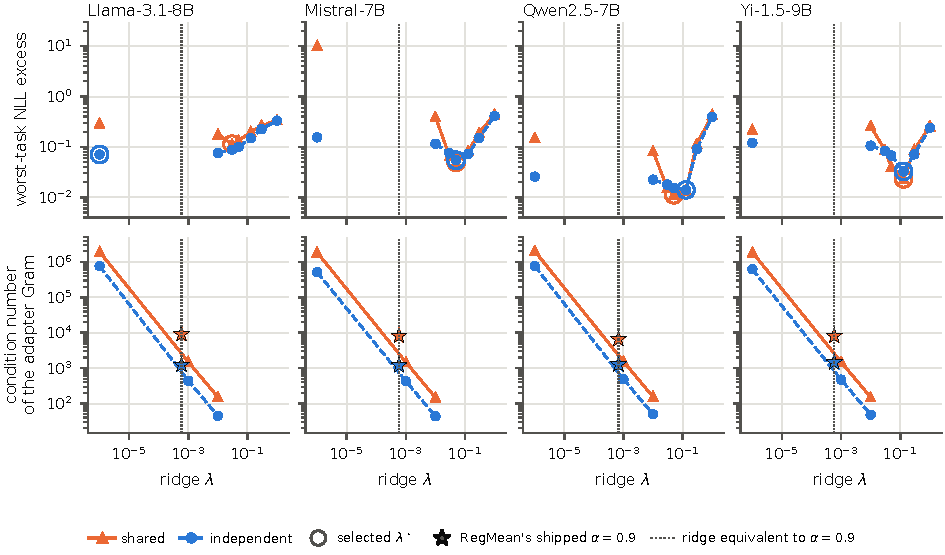
\includegraphics[width=\textwidth]{nc/figures/fig6_ridge.pdf}
\caption{Adapter-only RegMean against an added isotropic ridge $\lambda$, per
base model, on one shared and one independent cohort. \textbf{Top:} worst-task
NLL excess; circles mark the selected $\lambda^\star$, and the point at
$\lambda = 10^{-6}$ is not joined to the rest because no grid point lies
between. \textbf{Bottom:} condition number of the adapter Gram. Stars mark
RegMean's shipped $\alpha = 0.9$, placed at the isotropic ridge of the same
average size, $(1-\alpha)/\alpha$ times the mean diagonal of the Gram (dotted). That
size is the same on both arms, and on the shared arm it leaves a higher
condition number than an isotropic ridge of that size would.}
\label{fig:ridge}
\end{figure}

\subsection{A vision model, and all four tasks}\label{subsec:beyond}

\paragraph{A vision model.} We repeated the central comparisons on CLIP
ViT-B/32 with eight image classification tasks (SUN397, Cars, RESISC45,
EuroSAT, SVHN, GTSRB, MNIST and DTD). We trained rank-$16$ adapters in three
shared and three independent cohorts, merged them as dense updates without
truncation, and scored mean top-1 accuracy over the eight tasks. Every
registered prediction holds. The shared cohorts sit at median cosine $0.96$
and the independent ones at $0.11$. Adapter-only RegMean at
$\lambda = 10^{-6}$ scores $0.043$ on shared cohorts against $0.369$ on
independent ones, and at RegMean's shipped $\alpha = 0.9$ it scores $0.049$
against $0.398$. A ridge of $\lambda = 0.1$, the best grid value on both arms,
repairs it ($0.735$ against $0.747$). Task arithmetic ($0.742$ against
$0.739$) and TIES ($0.721$ against $0.711$) are equivalent within two points.
Activation-Gram RegMean ($0.768$ against $0.770$) and TSV-M ($0.654$ against
$0.670$) show no effect past the gate. WUDI's closed form fails as it does on
language models, $0.045$ against $0.369$. Published WUDI does not fail here.
Shared cohorts merge \emph{better} with it, $0.454$ against $0.358$, a
difference well past the gate and in the opposite direction to the language
models. Our registration asked only for the absence of harm, so this outcome
satisfies it. We did not predict a reversal, however, and cannot explain it,
and it is the clearest open question in this paper about the exposed class.

\paragraph{All four tasks.} The accuracy results so far cover mathematics and
code. We registered tests on the other two tasks: WMT19 English-to-German
(chrF on $500$ pairs) and IFEval (strict prompt-level accuracy on $300$
prompts). They use the seed-1 and independent-1 cohorts and our encoder, whose
merges at $\lambda = 0$ and at the selected $\lambda^\star$ were already
evaluated on the other tasks. On translation the collapse is visible. On the
shared cohort the selected ridge beats $\lambda = 0$ by $13.9$, $55.1$, $2.9$
and $6.5$ chrF points on the four bases, past the gate of $2$ on all four,
while task arithmetic and TIES differ across arms by at most $1.1$ points. On
IFEval it is not visible. The ridge gains $0.080$, $0.333$, $0.043$ and
$0.040$, past the gate on Mistral only; Llama misses by $0.001$ and is counted
as a miss, as registered. The heuristics again differ by at most $0.057$,
inside every gate. The reference rows account for part of this. The
instruction adapter alone does not beat the base model on IFEval on three of
four bases (Llama scores $0.627$ against the base model's $0.703$), so there
is little task skill for a broken merge to lose. The translation adapter is
also below the base model on chrF on three bases, the data-loading defect of
\S\ref{subsec:setup}. What the unregularised merge destroys on translation is
therefore mostly the base model's own ability to translate.

\subsection{Setting the ridge without data}\label{subsec:lambda}

A ridge repairs both solvers built from the adapter factors on most bases,
but the amount needed does not track the conditioning. We tested three data-free rules for choosing it, and all three
failed. The first sets $\lambda$ to bring the adapter Gram to a target
condition number, chosen in advance and evaluated only on unseen cohorts. It
was worse than a fixed $\lambda = 0.01$ on every collapsed cohort tested. On
separated cohorts it met its registered criterion of doing no harm on $4$ of
$6$, the two misses being cohorts where it did better than the minimal ridge,
and on collapsed public cohorts it brought the solver within $1.5$ times task
arithmetic's excess on $2$ of $6$, against a registered $80\%$. The fixed
$\lambda = 0.01$, registered to do the same on at least $80\%$ of collapsed
public cohorts, did so on $1$ of $6$.
Adapter-only RegMean is a ridge regression whose samples and targets can both
be read off the adapter files, so the classical parameter-choice rules apply as
they stand, and we registered generalised cross-validation (GCV) and the
L-curve. Neither repaired the collapse on more than one base of four, and
neither passed any of its three other registered criteria (no worse than
$\lambda = 0.01$, near the best of the sweep, no harm on separated cohorts);
GCV raised the independent cohort's excess on Llama from $0.07$ to $0.19$. GCV
chose $\lambda$ near $10^{-4}$ on shared cohorts and left the worst-task
excess at $1.13$, $8.66$, $0.22$ and $0.45$, against $0.11$, $0.05$, $0.01$
and $0.02$ at the best $\lambda$ of the sweep. On Llama, Qwen and Yi that is
worse than the minimal ridge. The L-curve found no interior corner: on every
base and arm its median choice was $1.3\times10^{-8}$, at the lower edge of a
grid that starts at $10^{-8}$. A data-free way to set the ridge
remains open. We recommend starting at $0.01$ and sweeping on held-out data.

\subsection{Public cohorts}\label{subsec:against}

\paragraph{On public cohorts the solver fails in both regimes.} We merged the
public cohorts that a fixed rule selected (causal language models of at most
$15$B parameters that load without custom code, members sharing rank and
target modules): seven collapsed and thirteen separated, of which one
collapsed cohort could not be loaded. Since public adapters rarely ship their
data, the consequence measure scored each adapter's own greedy completions on
a fixed prompt set under the merged model. Unregularised adapter-only RegMean
at least doubles task arithmetic's excess on $5$ of $6$ collapsed cohorts and
also on $11$ of $13$ separated ones (Fisher's exact test, $p = 0.78$). The
solver fails often on public cohorts, but not more often when they are
collapsed. These merges therefore show how common the collapse is
(\S\ref{sec:prevalence}), not what it costs on public cohorts.

\paragraph{Two candidate causes, tested on our own cohorts.} Public cohorts
differ from ours in ways a fixed rule cannot control, so we injected each
difference into our separated cohorts on Llama and Qwen. A LoRA update is
unchanged when $A$ is multiplied by $4$ and $B$ divided by $4$, but $A^\top A$
is not. That rescaling changes adapter-only RegMean's excess by at most $4\%$,
below the gate, so this factorisation freedom is not the cause, and putting
every adapter in a balanced form changes nothing either. Scale mismatch does
matter, which we did not predict. Making one adapter's update $4$ times larger
multiplies RegMean's excess by $3.9$ and $5.3$ on the two bases, while task
arithmetic's excess falls to $0.26$ and $0.29$ of its unperturbed value. Scale
mismatch between adapters is therefore a hazard specific to solvers, which we
observed on separated cohorts. It does not explain the public data, however: the spread of $A$ norms within a cohort is no larger where the
solver failed than where it did not. The public failures remain unexplained.

\subsection{The rule}\label{subsec:rule}

Across twelve methods, ten of them published methods we did not build, the
collapse reaches exactly the merges that solve a least-squares problem, in
closed form or by gradient descent, whose matrix is built from the adapters
alone: from their factors, or from the task updates they define. That class
includes a published method run exactly as its authors run it. The collapse
does not reach averaging or sparsifying merges, solvers whose matrix is built
from data, a diagonal solver, or whitening.


\section{Discussion and limitations}\label{sec:discussion}
\paragraph{What to do in practice.} The results reduce to three cases.
\begin{itemize}[leftmargin=*,itemsep=1pt,topsep=2pt]
\item If the merge averages or sparsifies the updates, or is a solver whose
  matrix is built from data, the initialisation does not matter and no action
  is needed.
\item If the merge solves a least-squares problem whose matrix is built from
  the adapters alone, as adapter-only RegMean, WUDI-Merging and our encoder
  do, run Algorithm~\ref{alg:audit} first. On a separated cohort these merges
  behave as intended. On a collapsed one, add an isotropic ridge to the
  closed-form solvers, start near $\lambda = 0.01$ and sweep it on held-out
  data, and do not rely on RegMean's shipped $\alpha$. We did not test a
  repair for WUDI as published; running it ten times longer makes it worse or
  no better (Table~\ref{tab:wudi}), so on a collapsed cohort we would use one
  of the unaffected merges instead.
\item If several tasks are fine-tuned with Unsloth or LLaMA-Factory at default
  settings, or each from one existing adapter, the adapters are collapsed; so
  is a PiSSA cohort whatever its seeds, and OLoRA and MiLoRA start every task
  from the same $A$ in the same way. A different seed per task avoids the first
  case and not the others. Designs that share $A$ deliberately, such as
  HydraLoRA or federated LoRA with a frozen or aggregated $A$, are collapsed by
  construction.
\end{itemize}
The audit is worth running even though a ridge repairs most of the damage. A
sweep needs held-out data and one merge per value of $\lambda$, and none of the
three data-free rules we tested sets $\lambda$ well (\S\ref{subsec:lambda}). A
user who has no data for the tasks, or who runs a method at its defaults, meets
the zeros of Table~\ref{tab:wudi} and Figure~\ref{fig:exposure} with no
warning. The audit needs only the $A$ factors and a CPU minute, and it says
before any merge whether the choice of method matters at all.

\paragraph{Predictions that failed.} Each registered prediction that did not
hold is reported where it arises. Grouped by what they cost, they are these.
Four changed what this paper claims. Published WUDI was predicted to be
protected by its early-stopped optimiser, and it is not, in NLL or in accuracy;
this is the lead result (\S\ref{subsec:wudi}). TSV-M was predicted to be
exposed and is not, so the rule is stated for least-squares merges alone
(\S\ref{subsec:results}). The collapse was predicted to be visible on all four
tasks and is invisible on IFEval, where the instruction adapter has little
skill to lose (\S\ref{subsec:beyond}). Solver failures on public cohorts were
predicted to be specific to the collapse and are not (\S\ref{subsec:against}).

Six were explanations that did not survive. The closed form of WUDI does not
concentrate its energy in the ill-conditioned directions, and the 3000-step arm
does not lie between the other two on two of the four bases
(\S\ref{subsec:wudi}). The heuristics' slight lean towards the shared arm did
not vanish at three cohorts per arm, and merging without truncation did not
halve it (\S\ref{subsec:results}). Neither the factorisation freedom of LoRA
nor the spread of adapter norms explains the public failures
(\S\ref{subsec:against}).

Three were tools. A rule that sets the ridge by a target condition number did
worse than a fixed $\lambda = 0.01$, and generalised cross-validation and the
L-curve each repaired the collapse on at most one base of four
(\S\ref{subsec:lambda}).

Three more concern details. A fourfold scale mismatch between adapters was
predicted not to be specific to solvers, and it multiplies the solver's excess
by $3.9$ and $5.3$ while lowering that of task arithmetic
(\S\ref{subsec:against}). RegMean with activation Grams produced solutions
$2.2$ to $6.5$ times the mean task update rather than at most three, equally on
both arms, because the activation Grams are themselves badly conditioned
($10^{4}$ to $10^{7}$) whatever the initialisation. The retrained translation
adapter improved but did not become the best adapter at translation.

\paragraph{What we cannot explain.} Three observations have no tested
explanation. On CLIP ViT-B/32, published WUDI merges shared cohorts
\emph{better} than independent ones, $0.454$ against $0.358$, the opposite of
its behaviour on language models (\S\ref{subsec:beyond}); the description we
give in \S\ref{subsec:wudi}, in which Adam's steps leave the row space on a
collapsed cohort, does not account for it. Scaling the initial $A$ by $0.25$
leaves a cohort collapsed, yet adapter-only RegMean then does less damage than
on the independent arm ($0.022$ against $0.071$ nats), at the same
$\kappa(\bar H)$ as a cohort where it does a great deal (\S\ref{sec:theory}).
That points at the amplification rather than the condition number as what a
solver responds to, but it rests on two cohorts. And the heuristics' lean of
$0.7$ points towards the shared arm, like the solver failures on public
cohorts, survives every explanation we tested.

\paragraph{Relation to the earlier version.} The preprint this paper
supersedes~\citep{pathak2026rd} reported that our closed-form encoder had the
lowest worst-task loss of ten methods on all four bases. That advantage came
from the shared initialisation of its cohorts: on independent cohorts the
encoder beats the best baseline on no base. It also reported that worst-task
NLL tracks the downstream ranking of methods. With five or six methods that
correlation cannot be measured reliably, and on HumanEval its sign is wrong,
which is why every accuracy claim here is measured in accuracy.

\paragraph{Limitations.} The controlled experiments use four base models of 7
to 9 billion parameters and four tasks, one of which did not train properly,
so the merged models contain one weak member. The seed ablation, the
task-count and rank sweep and the out-of-sample test of the scalar law are on
one base; the vision replication is one model; DoRA was measured in geometry
only. Larger models, other architectures and other adapter types are untested.
The value of $\kappa(\bar H)$ depends on the projector curvature model, while
the principal cosines, which carry the audit, are independent of it. The
theory is a leading-order expansion verified numerically, not a bound. The
float32 values we report for the unregularised encoder on shared cohorts are
single draws, which move by $0.02$ to $0.08$ nats between draws
(\S\ref{sec:merging}). The tests on translation and IFEval use one cohort per
arm, so their nulls are at the resolution of the gate. Training and evaluation
data overlap on two tasks ($13$ to $16\%$ for instruction following and $9$ to
$12\%$ for code), so absolute scores are optimistic; every comparison here is
between the two initialisation arms on the same data, and on the disjoint
subset the ordering of methods is unchanged in $19$ of $20$ cases. The library
reading is of pinned versions, and defaults can change. The prevalence of
$40\%$ is among public cohorts as the sampling frame defines them, and most of
the collapsed ones are versions of one model rather than tasks one would merge
(\S\ref{subsec:public}). Finally, adapter-built solvers fail often on released
adapters for reasons we have not identified; those failures should not be
attributed to the collapse, and such solvers should not be used on public
adapters without checking the result.


\section{Conclusion}\label{sec:conclusion}
Whether the adapters of a LoRA cohort share their initial $A$ is fixed before
training starts, is decided by a seed or a library default, and is almost never
reported. It changes the cohort's geometry by orders of magnitude: shared
starts leave the task subspaces nearly collinear, and a first-order theory in
the adapters' displacement predicts the resulting conditioning of the merge
operator to within $0.11\%$. The collapsed regime is common, in our own
pipelines, in two popular fine-tuning stacks at their defaults, in PiSSA-style
initialisations whatever the seed, and in $17$ of $45$ public cohorts. Its
consequences for merging are specific: averaging, sparsifying and data-built
merges are unaffected, while solvers built from the adapters' own factors fail
and need a ridge that the shipped default does not supply. A one-minute audit
of the adapter files tells which case a cohort is in.

\paragraph{Code and data availability.} The code, configurations, per-cell
results, pre-registration documents and the commit history that orders them
are public at \url{\repourl}, including the audit script
(\texttt{measure\_\allowbreak subspace\_\allowbreak geometry.py}).


% CRediT roles come from the \credit tags in the front matter.
\printcredits

% Elsevier end matter. All three author decisions (Singh's CRediT roles, the
% funding statement, the AI declaration) were confirmed by the corresponding
% author on 2026-10-06. Elsevier's June 2026 AI policy also requires AI-assisted
% code to be declared in the Methods; that sentence is in nc/s3_collapse.tex.

% The CRediT statement is printed by \printcredits from the \credit tags in
% the front matter of neurocomputing.tex (CAS class); it is not repeated here.

\section*{Declaration of competing interest}
The authors declare that they have no known competing financial interests or
personal relationships that could have appeared to influence the work reported
in this paper.

\section*{Funding}
This research did not receive any specific grant from funding agencies in the
public, commercial, or not-for-profit sectors.

\section*{Data availability}
All code, configurations, per-cell results, the pre-registration documents and
the commit history that orders them are public at \url{\repourl}. The trained
adapters are available from the authors on request; the base models and
datasets are public.

\section*{Declaration of generative AI and AI-assisted technologies in the
writing process}
During the preparation of this work the authors used Claude (Anthropic) in
order to produce initial versions of the code for some parts of the experiments
and analyses, to organise the manuscript, and to draft and edit text from the
authors' own analyses, decisions and earlier manuscript. After using this tool, the authors reviewed
and edited the content as needed and take full responsibility for the content
of the publication.

\section*{Acknowledgements}
We thank Jaypee Edusphere for access to its supercomputing facility, Ramanujan
Universe, on which the more than $400$ GPU-hours of A100-80GB compute reported
here were carried out, and the anonymous reviewers of earlier versions of this
work.


\bibliographystyle{elsarticle-num-names}
\bibliography{references}

\appendix
\section{Derivation of the first-order theory}\label{app:theory}
This appendix derives Proposition~\ref{prop:drift}. Throughout, $W_0$ is an
orthonormal basis of the row space of $A_0$, $P_\perp = I - W_0W_0^\top$, and
the tilts $X_t$ of \eqref{eq:tilt} satisfy $W_0^\top X_t = 0$.

\paragraph{Projectors.} The columns of $W_0 + X_t$ span $V_t$ and have Gram
matrix $I + X_t^\top X_t$, so exactly
\[
  P_t = (W_0 + X_t)\,(I + X_t^\top X_t)^{-1}\,(W_0 + X_t)^\top .
\]
In the orthogonal decomposition $\R^d = \operatorname{col}(W_0) \oplus V_0^\perp$,
with $C_t = (I + X_t^\top X_t)^{-1} = I - X_t^\top X_t + O(\|X_t\|^4)$, the
operator $\bar H = \frac1T\sum_t P_t$ has the block form
$\bigl(\begin{smallmatrix} H_{00} & H_{10}^\top \\ H_{10} & H_{11}
\end{smallmatrix}\bigr)$ with
\begin{align*}
  H_{00} &= \tfrac1T\textstyle\sum_t C_t = I - O(\|X\|^2), \\
  H_{10} &= \tfrac1T\textstyle\sum_t X_t C_t = \bar X + O(\|X\|^3), \\
  H_{11} &= \tfrac1T\textstyle\sum_t X_t C_t X_t^\top
          = \tfrac1T\textstyle\sum_t X_t X_t^\top + O(\|X\|^4).
\end{align*}

\paragraph{Eigenvalues.} The top-left block is $I - O(\|X\|^2)$, which
accounts for $r$ eigenvalues near $1$. The remaining nonzero eigenvalues are,
to leading order, those of the Schur complement on $V_0^\perp$,
\begin{align*}
  S &= \tfrac1T\textstyle\sum_t X_tX_t^\top - \bar X\bar X^\top + O(\|X\|^4) \\
    &= \tfrac1T\textstyle\sum_t (X_t - \bar X)(X_t - \bar X)^\top + O(\|X\|^4)
     = \Sigma_X + O(\|X\|^4),
\end{align*}
whose rank is at most $(T-1)r$ because the centred tilts sum to zero. With
$Tr \le d$ and the tilts in general position this rank is attained, so
$\bar H$ has $Tr$ nonzero eigenvalues, $r$ near $1$ and $(T-1)r$ equal to those
of $\Sigma_X = \tfrac1T YY^\top$ to leading order, and
$\kappa(\bar H) \approx 1/\lambda^{+}_{\min}(\Sigma_X) = T/\sigma_{\min}(Y)^2$.

\paragraph{The interpolator.} Each update lies in its own row space,
$D_t = D_tP_t$, so the exact interpolator $\tauH = \bar D \bar H^{+}$ is the
minimum-norm $w$ in $\range(\bar H)$ with $w\,(W_0 + X_t) = D_t(W_0 + X_t)
= M_t$ for every $t$. Writing $w = aW_0^\top + b$ with $b = wP_\perp$, the
conditions read $a + bX_t = M_t$. Averaging gives $a = \bar M - b\bar X$;
subtracting the average gives $b\,(X_t - \bar X) = M_t - \bar M$ for all $t$,
that is $bY = [M_1 - \bar M, \dots, M_T - \bar M]$, whose minimum-norm solution
in the span of the tilts is $b = [M_t - \bar M]_t\,Y^{+}$. Minimising
$\|a\|^2 + \|b\|^2$ jointly couples $a$ and $b$ through $\bar X$; dropping that
coupling is the only approximation in item~2 and costs a relative
$O(\|\bar X\|)$, which vanishes for the consensus choice of $W_0$ used in the
reference-free test.

\paragraph{Scaling.} Under $E_t \mapsto sE_t$ the tilts scale as
$X_t \mapsto sX_t + O(s^2)$, so $\Sigma_X \mapsto s^2\Sigma_X$ and
$\kappa \propto s^{-2}$. The differences $M_t - \bar M$ are dominated by the
differences between the $B_t$, which do not scale with $s$, so
$\|b\| \propto s^{-1}$. Since $\|b\|$ dominates $\|\tauH\|$ in the collapsed
regime and $\|\bar D\|$ is $O(1)$ in $s$, the amplification scales as
$s^{-1}$.

\paragraph{Numerical checks beyond the registered ones.} On synthetic cohorts
($d = 512$, $r = 16$, $T = 4$) with isotropic and with low-rank anisotropic
displacements, the formulas match the exact quantities to within $0.3\%$. The
anisotropic case reproduces $\kappa \sim 10^{5}$ to $10^{6}$ at the same
$\varepsilon$ that gives $\kappa \sim 5\times10^{2}$ in the isotropic case,
which is the mechanism behind the second consequence in \S\ref{sec:theory}.


\section{Pre-registration and commit trail}\label{app:prereg}
Every confirmatory test in this paper is governed by a registration document
committed to version control before the compute it governs was run. Each
document states the predictions, the decision rule, and the consequence text
for every possible outcome, including the outcomes that would cost us a claim.
Thresholds were never moved after data were seen, and analyzers refuse to
report until every cell they need exists. Analyses that were not registered,
such as the seed follow-ups of the precision check, are labelled as such in
the text; their plans were committed before their cells ran.

The registration documents are the files \texttt{notes/prereg\_*.md} of the
public repository, at \url{\repourl}; the August ones are also in
\texttt{paper/prereg/}. The precision check's rule and result,
\texttt{notes/check\_solve\_precision\_2026-10-24.md} and its
\texttt{\_result} companion, are reachable at the commits in its row.
Table~\ref{tab:commits} gives, for each registration this paper relies on, the
commit that fixed its rules, the commit that added the generator or
implementation, and the commit that added the result. A reader can check any
row with
\begin{center}
\texttt{git merge-base -{}-is-ancestor <rules> <result>}
\end{center}
which exits zero exactly when the rules commit precedes the result. The hashes
are those of the public repository, whose history is filtered to remove
private correspondence and large build artifacts and to replace the names of
our compute account and host wherever they occur; that replacement changes
one line in each of the October registrations and no number. Filtering
rewrites hashes but not the order of commits, which is what the check depends
on. Hashes cited inside the registration documents themselves are those of
our working repository at the time and do not resolve publicly; we leave them
unedited, since an unedited document is the point.

\begin{table}[pos=h]
\centering
\small
\caption{Commit trail for the registrations behind this paper, in the public
repository's hash space.}
\label{tab:commits}
\begin{tabular}{p{5.2cm}llp{2.2cm}l}
\toprule
registration & section & rules & generator & result \\
\midrule
drift of $A$ across training & \S\ref{subsec:why} & \texttt{8544b36} & \texttt{0c8770b} & \texttt{5e01813} \\
replication on independent cohorts & \S\ref{subsec:results} & \texttt{9b3f57e} & --- & \texttt{4328446} \\
conditioning and the ridge & \S\ref{subsec:results} & \texttt{dc0a1f1} & \texttt{ac4499f}, \texttt{25d4d47} & \texttt{efa1d2d} \\
untruncated merges (encoder) & \S\ref{subsec:results} & \texttt{876fcb6} & \texttt{e4043b4} & \texttt{63bdf0c} \\
shared arm at three cohorts & \S\ref{subsec:results} & \texttt{3b9db2f} & \texttt{7c25aa1} & \texttt{0a4afaf} \\
public-cohort prevalence & \S\ref{subsec:public} & \texttt{335a4f6} & \texttt{0b6eb40} & \texttt{0a4afaf} \\
downstream accuracy & \S\ref{subsec:results} & \texttt{a56b31e} & \texttt{321a808} & \texttt{0a4afaf} \\
\addlinespace
first-order theory & \S\ref{sec:theory} & \texttt{b0c01a5} & \texttt{222e30b} & \texttt{58d987d} \\
RegMean with data, and adapter-only & \S\ref{subsec:results} & \texttt{a50ab11} & \texttt{b93b76f} & \texttt{400f499} \\
\quad amendment (Gram correction) & \S\ref{subsec:results} & \texttt{bf971af} & \texttt{bddcad9}, \texttt{383e8e3} & \texttt{58d987d} \\
heuristics equivalence & \S\ref{subsec:results} & \texttt{0265f64} & \texttt{bf80ff8} & \texttt{400f499} \\
TSV-M, MaTS, diagonal Fisher & \S\ref{subsec:results} & \texttt{c4f2e28} & \texttt{64741e5} & \texttt{58d987d} \\
task count, rank, PiSSA, translation & \S\ref{subsec:tr} & \texttt{67ec001} & \texttt{61ec804}, \texttt{dd952d5} & \texttt{58d987d} \\
public-cohort merges & \S\ref{subsec:against} & \texttt{1be9d9d} & \texttt{383e8e3}, \texttt{6dcd988} & \texttt{58d987d} \\
data-free ridge rule & \S\ref{subsec:lambda} & \texttt{d733f81} & \texttt{6dcd988}, \texttt{dd952d5} & \texttt{58d987d} \\
\addlinespace
WUDI-Merging & \S\ref{subsec:wudi} & \texttt{fff1699} & \texttt{0a2b64e}, \texttt{db8c994} & \texttt{c55e5d9} \\
ridge selection (GCV, L-curve) & \S\ref{subsec:lambda} & \texttt{fff1699} & \texttt{0a2b64e} & \texttt{9f3d827} \\
seed ablation, training regimes, routes & \S\ref{subsec:seeds}, \S\ref{sec:theory} & \texttt{fff1699} & \texttt{61b2dca} & \texttt{fe3bb6a} \\
\quad amendment (calibration) & \S\ref{sec:theory} & \texttt{50e490a} & \texttt{9fc0e5a} & \texttt{fe3bb6a} \\
vision (CLIP ViT-B/32) & \S\ref{subsec:beyond} & \texttt{fff1699} & \texttt{61b2dca} & \texttt{651edb5} \\
heterogeneity, partial collapse & \S\ref{subsec:audit}, \S\ref{subsec:against} & \texttt{fff1699} & \texttt{33c6f7c} & \texttt{1debb3f} \\
\quad prevalence re-read & \S\ref{subsec:public} & \texttt{fff1699} & \texttt{d11375d} & \texttt{d11375d} \\
truncation and the heuristics' lean & \S\ref{subsec:results} & \texttt{fff1699} & \texttt{33c6f7c} & \texttt{b1066d9} \\
all four tasks & \S\ref{subsec:beyond} & \texttt{fff1699} & \texttt{76353d5} & \texttt{3672064} \\
solve precision (float64) & \S\ref{subsec:results} & \texttt{9830e06} & \texttt{98ea4cc}, \texttt{dc65838} & \texttt{0e4a322} \\
\quad rebuild of the failing merge & \S\ref{subsec:results} & \texttt{0e4a322} & \texttt{6d436cf} & \texttt{58d5275} \\
\bottomrule
\end{tabular}
\end{table}

The amendment row records one error. Adapter-only RegMean was described
as using the Gram $\sum_t A_t^\top A_t$, but a missing hook made every earlier
run fall back to $\sum_t \Delta_t^\top\Delta_t$. We found this, registered an
amendment before any affected cell ran, fixed the hook and re-ran the results
under their original rules; both registered predictions still hold, and every
adapter-only RegMean number in this paper uses the described Gram.

Three rows of the October block need a word. The seven October registrations
share one rules commit, made before any of their code. The calibration
amendment changed how the constants of the scalar law were to be computed
before they were computed, and the constants were committed before any of the
cohorts they predict existed. The WUDI generator was corrected once, to
evaluate the registered loss from the adapter factors rather than densely,
before any WUDI cell finished, as the campaign log records; the two forms agree
in value and gradient. The
prevalence re-read adds its script and its result in one commit, after the
rules that required it. In the precision row the second generator commit fixes
a first run that compared two different truncation algorithms; that run was
void, and the result comes from the corrected one. The rebuild row's rules
commit is the precision result itself, which wrote the rebuild plan before any
rebuild cell was generated.


% Author biographies with photographs, required by Neurocomputing. Created
% once the three bios and photos arrive; see nc/author_bios.md.
\IfFileExists{nc/bios.tex}{\input{nc/bios}}{}

\end{document}
